% examples of appendices. **DO NOT PUT \end{document} at the end
 \clearpage
 \appendix
% \section{Additional plots}


 \begin{figure*}[h!]
     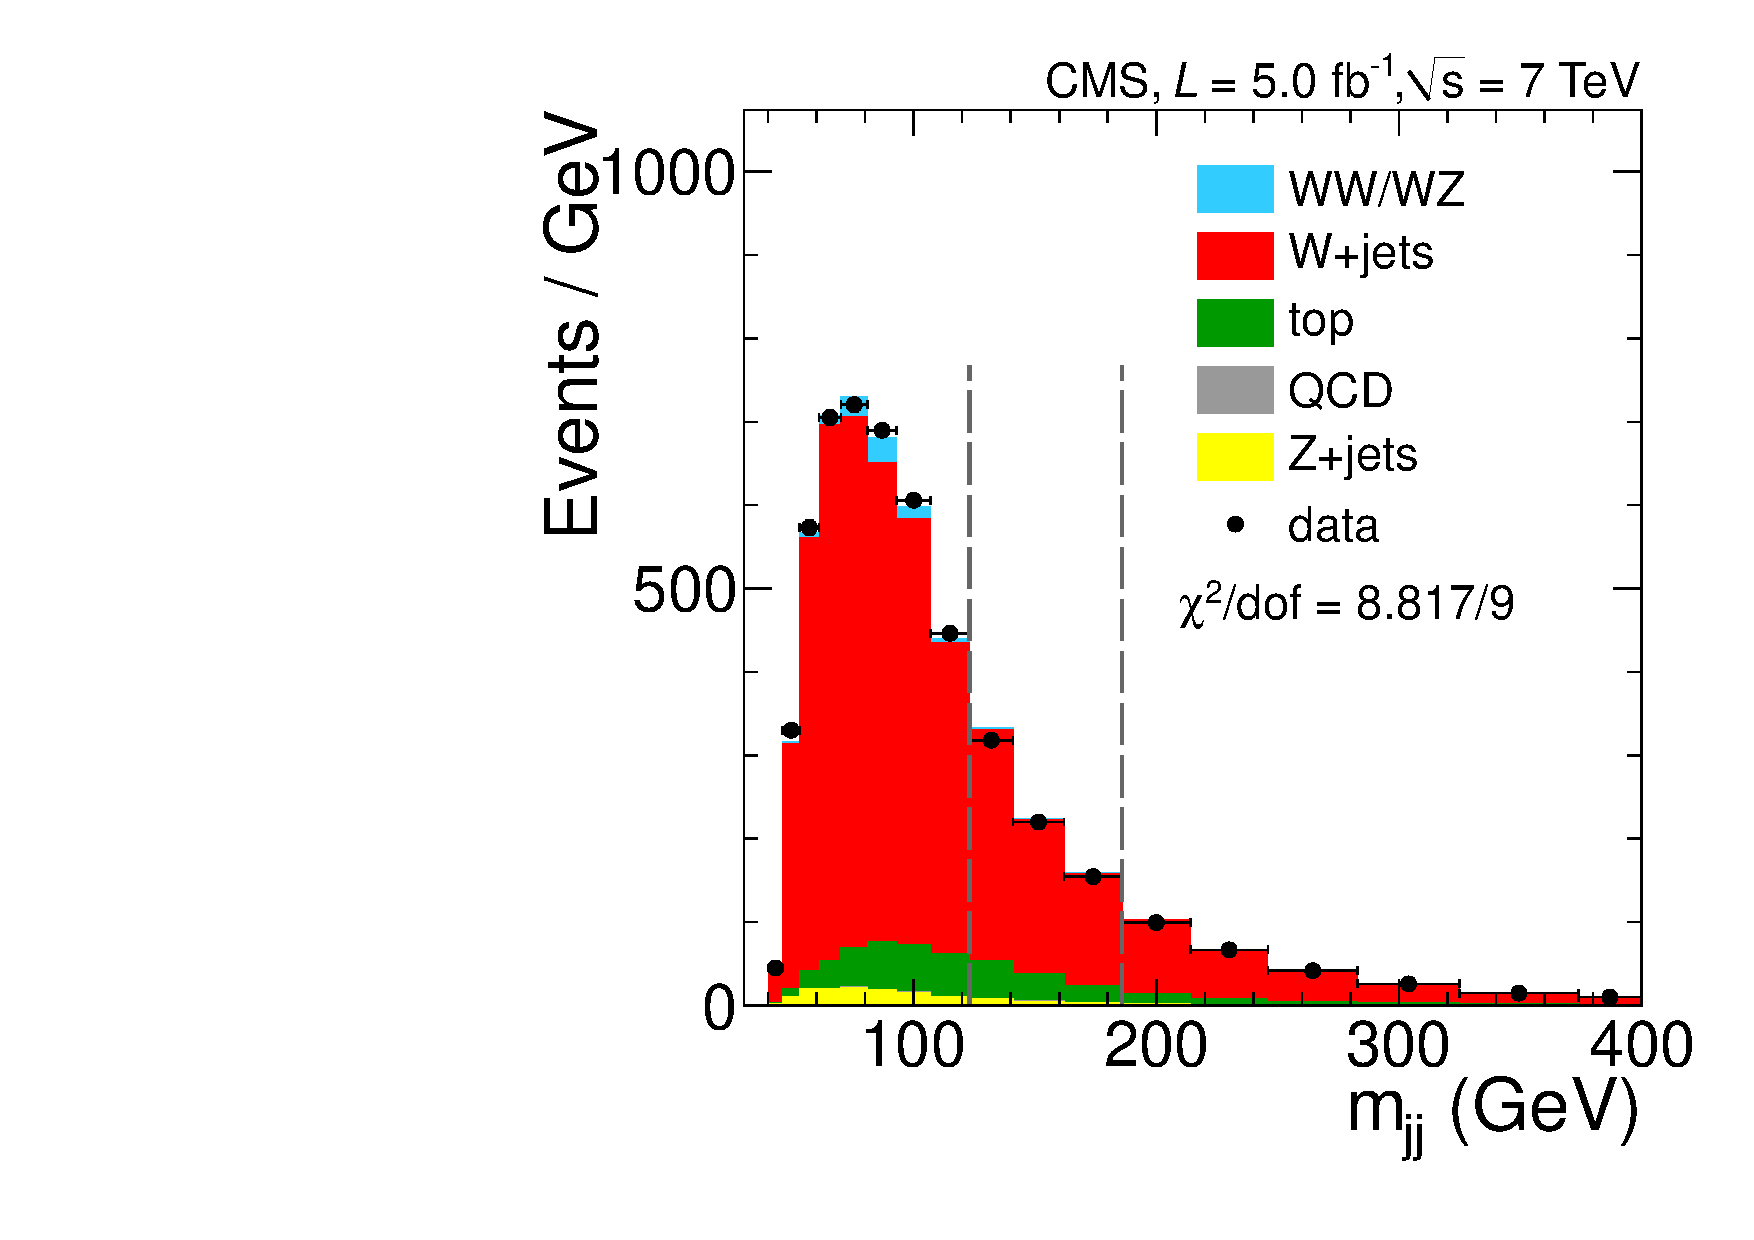
\includegraphics[width=0.49\textwidth]{figs/Wjj_Mjj_Muon_2jets_Stacked.pdf}
     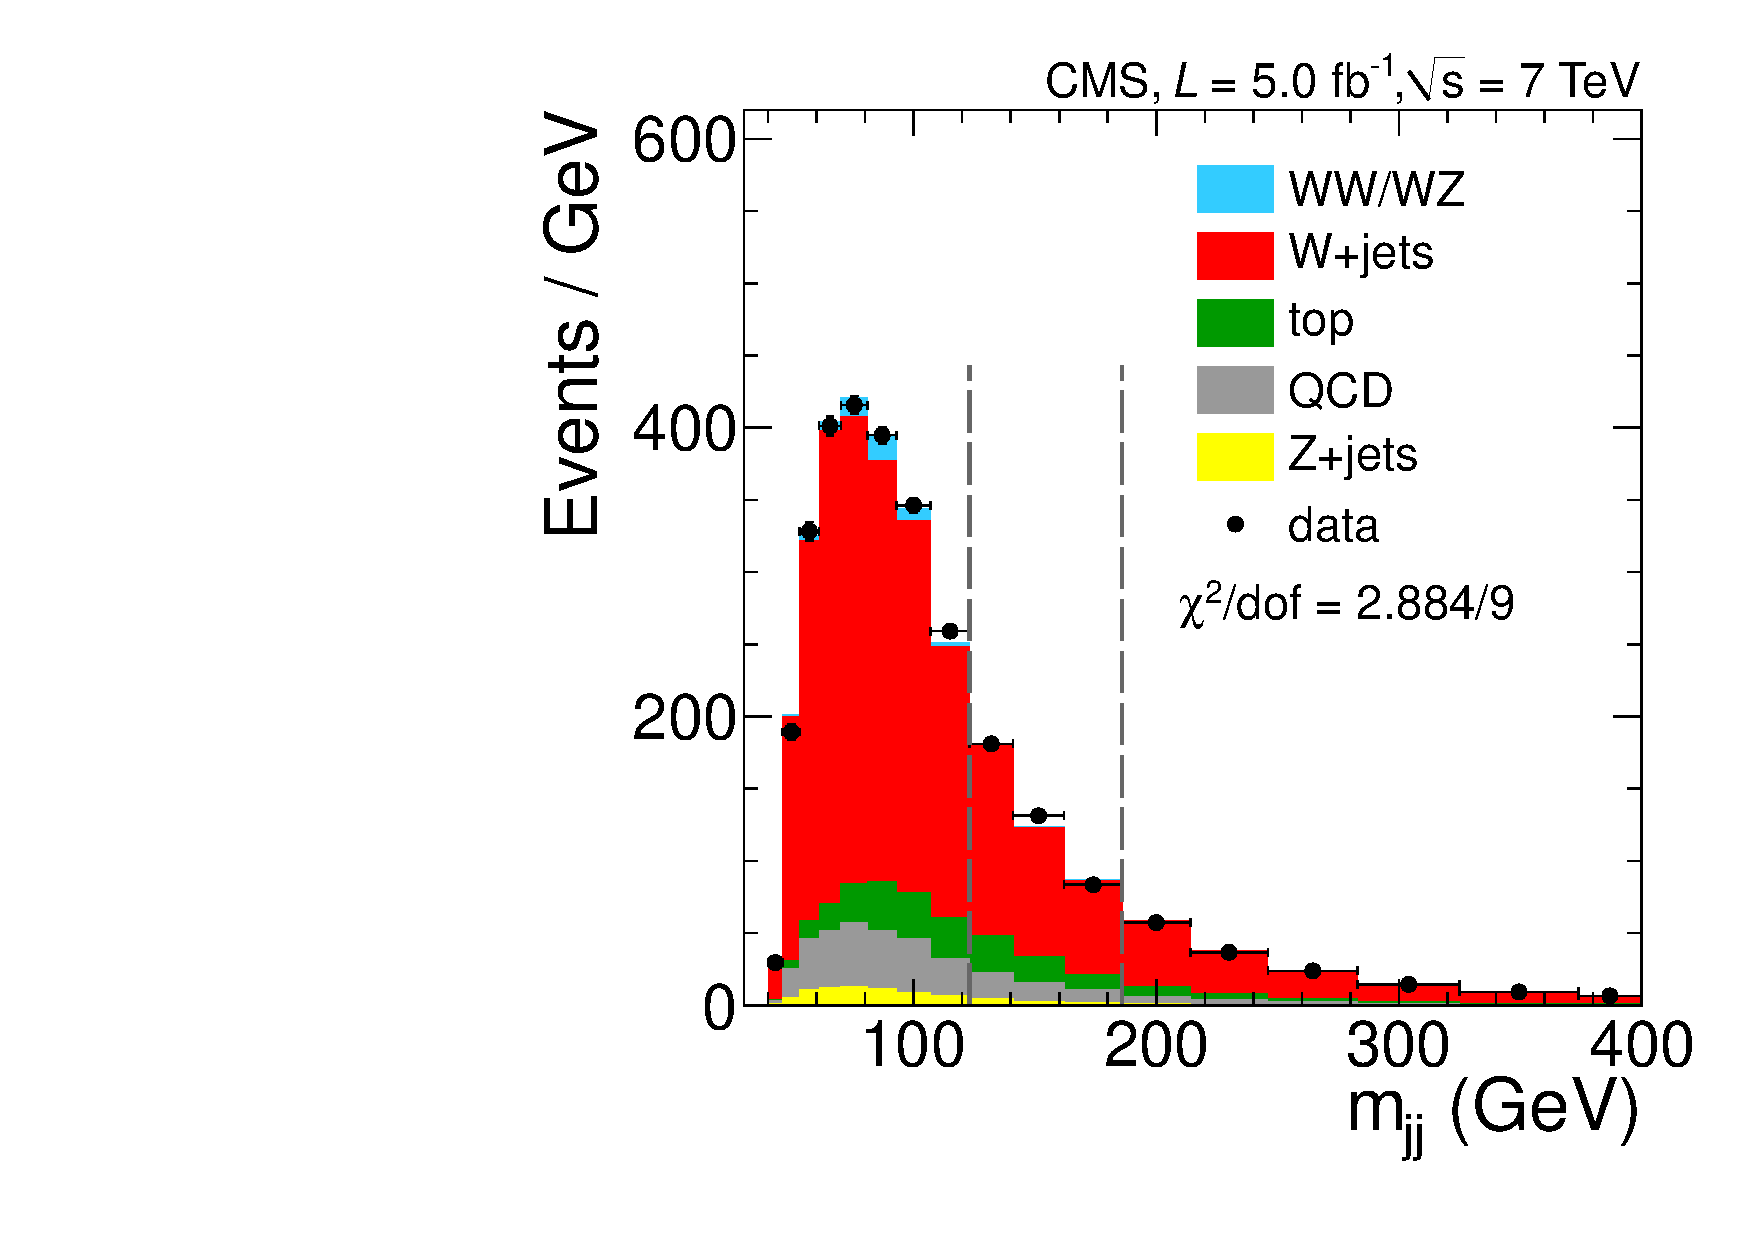
\includegraphics[width=0.49\textwidth]{figs/Wjj_Mjj_Electron_2jets_Stacked.pdf}
     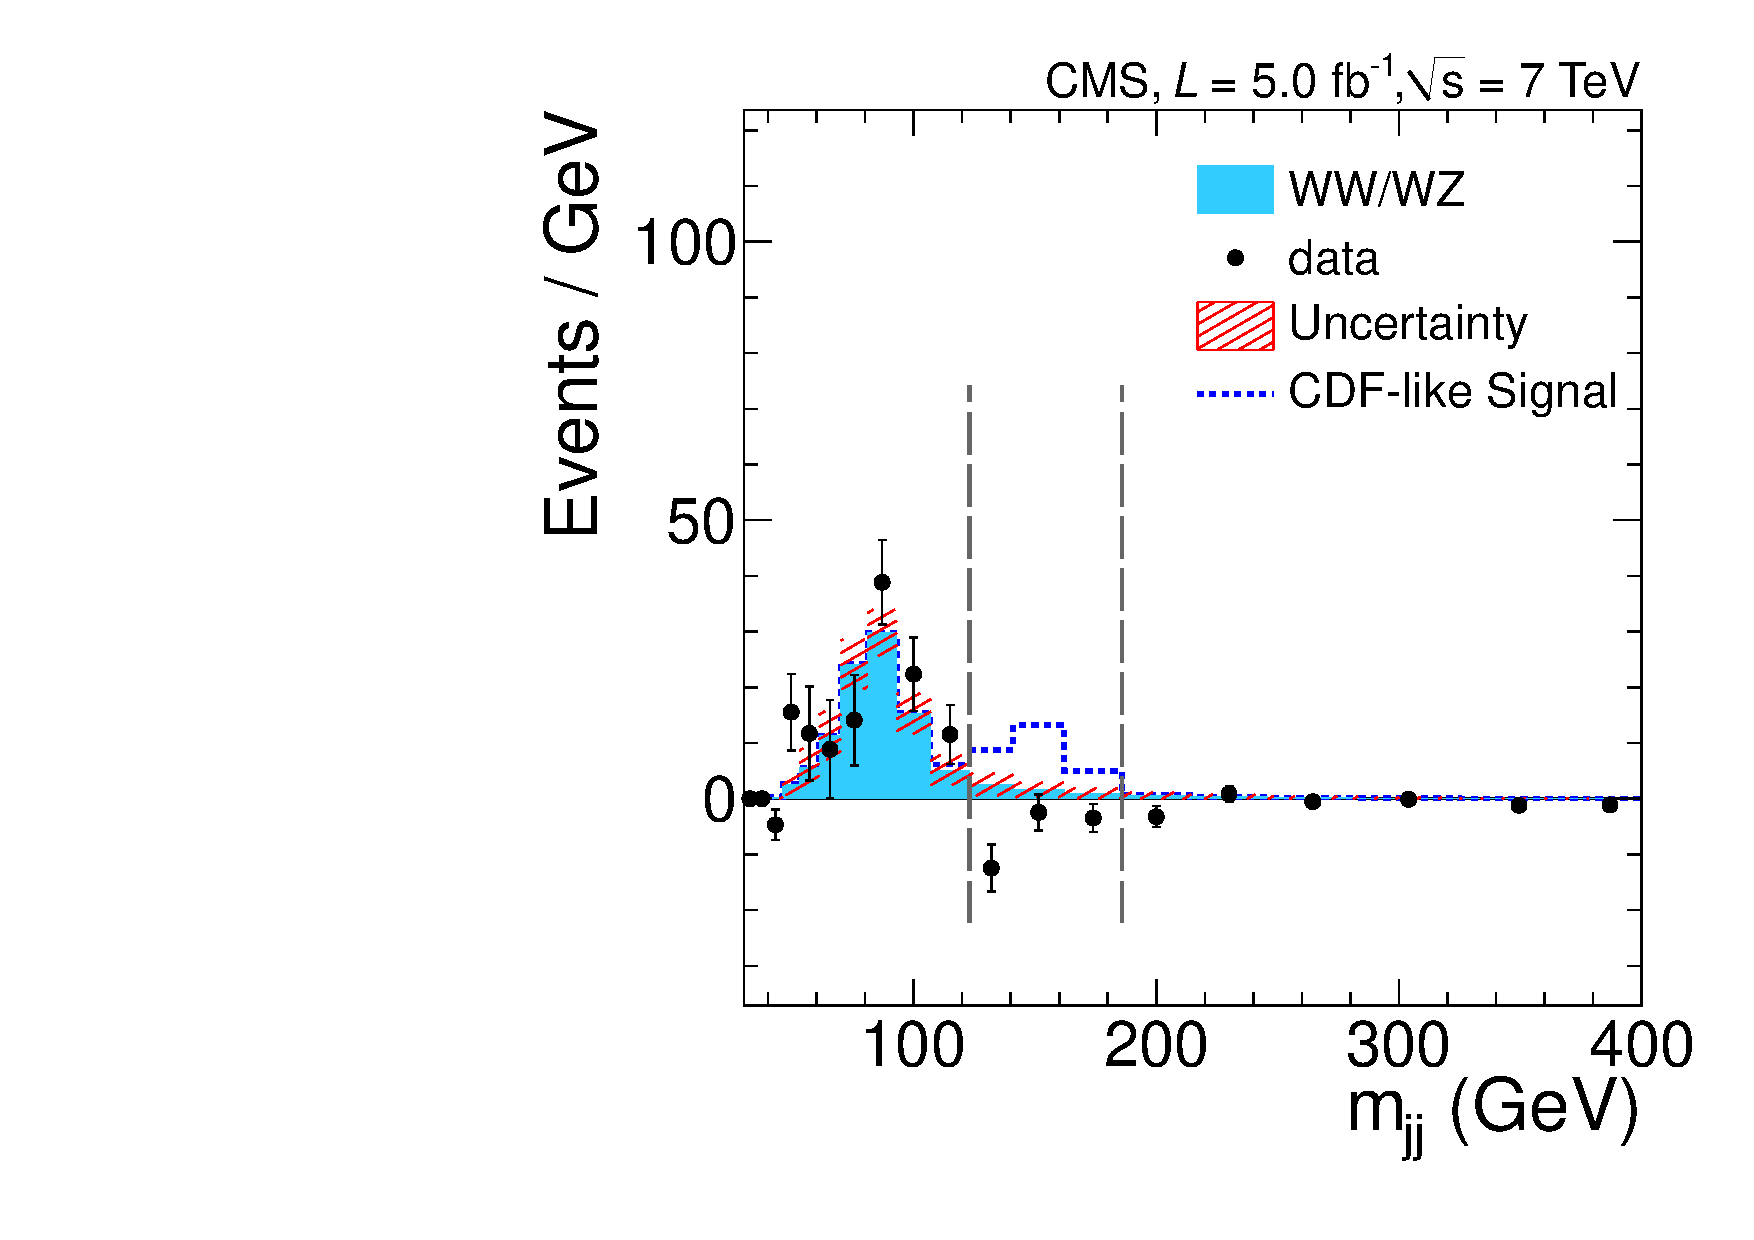
\includegraphics[width=0.49\textwidth]{figs/Wjj_Mjj_Muon_2jets_Subtracted.pdf}
     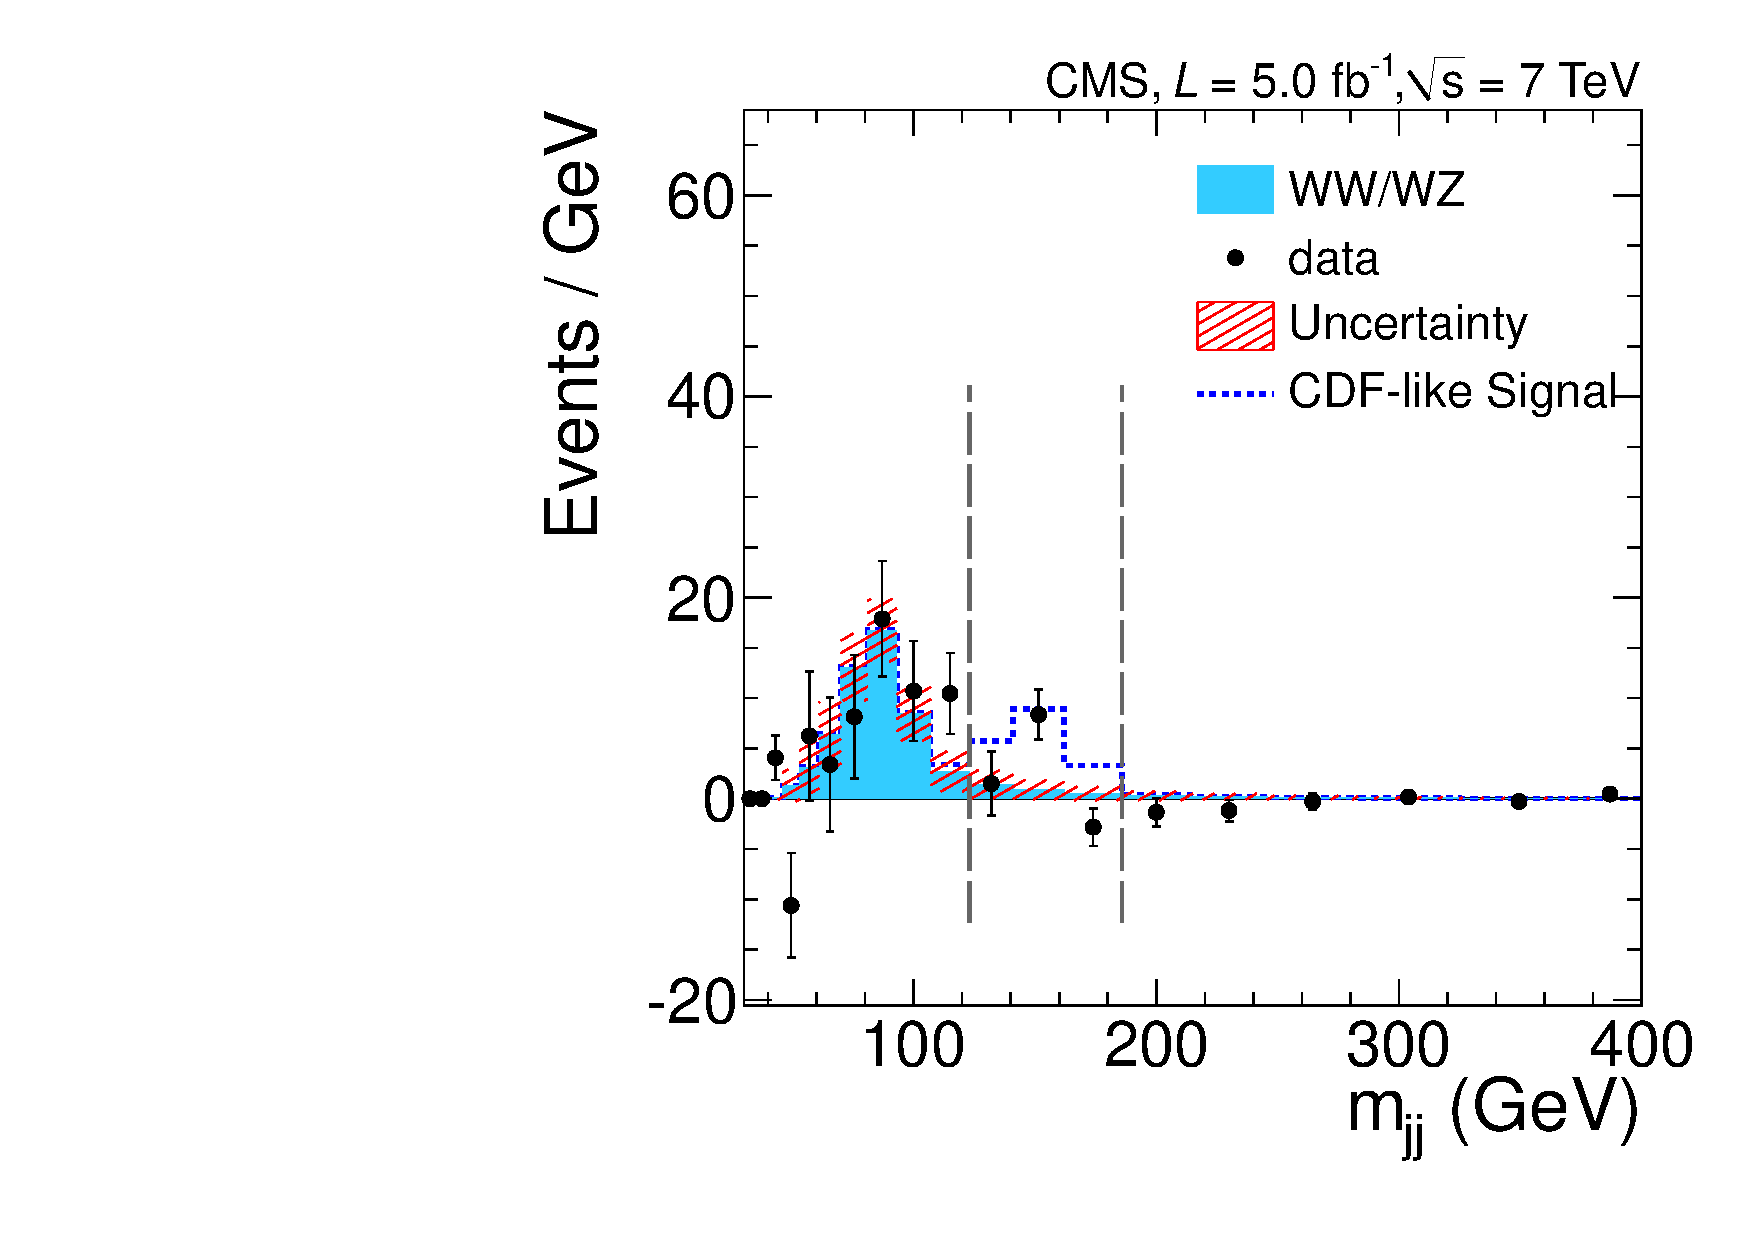
\includegraphics[width=0.49\textwidth]{figs/Wjj_Mjj_Electron_2jets_Subtracted.pdf}
   \caption{(upper row) Distribution of the invariant mass spectrum of
     the two jets observed in data in muon plus 2 jets (left) and
     electron plus 2 jets (right) categories.  Overlaid are the
     template distributions used in the likelihood fit to the measured
     \mjj distibution, with their relative normalization as obtained
     from the fit.  The region between the vertical dotted lines is
     excluded in the fit.  Depicted is the number of events per GeV,
     \textit{i.e.}, the raw event count can be obtained by multiplying
     with the bin width.  (lower row) The same distribution after
     subtraction of all SM components except the electroweak diboson
     WW/WZ.  Error bars correspond to the statistical uncertainty.
     The band represents the systematic uncertainty in the sum of the
     SM components. }
 \end{figure*}





 \begin{figure*}[h!]
   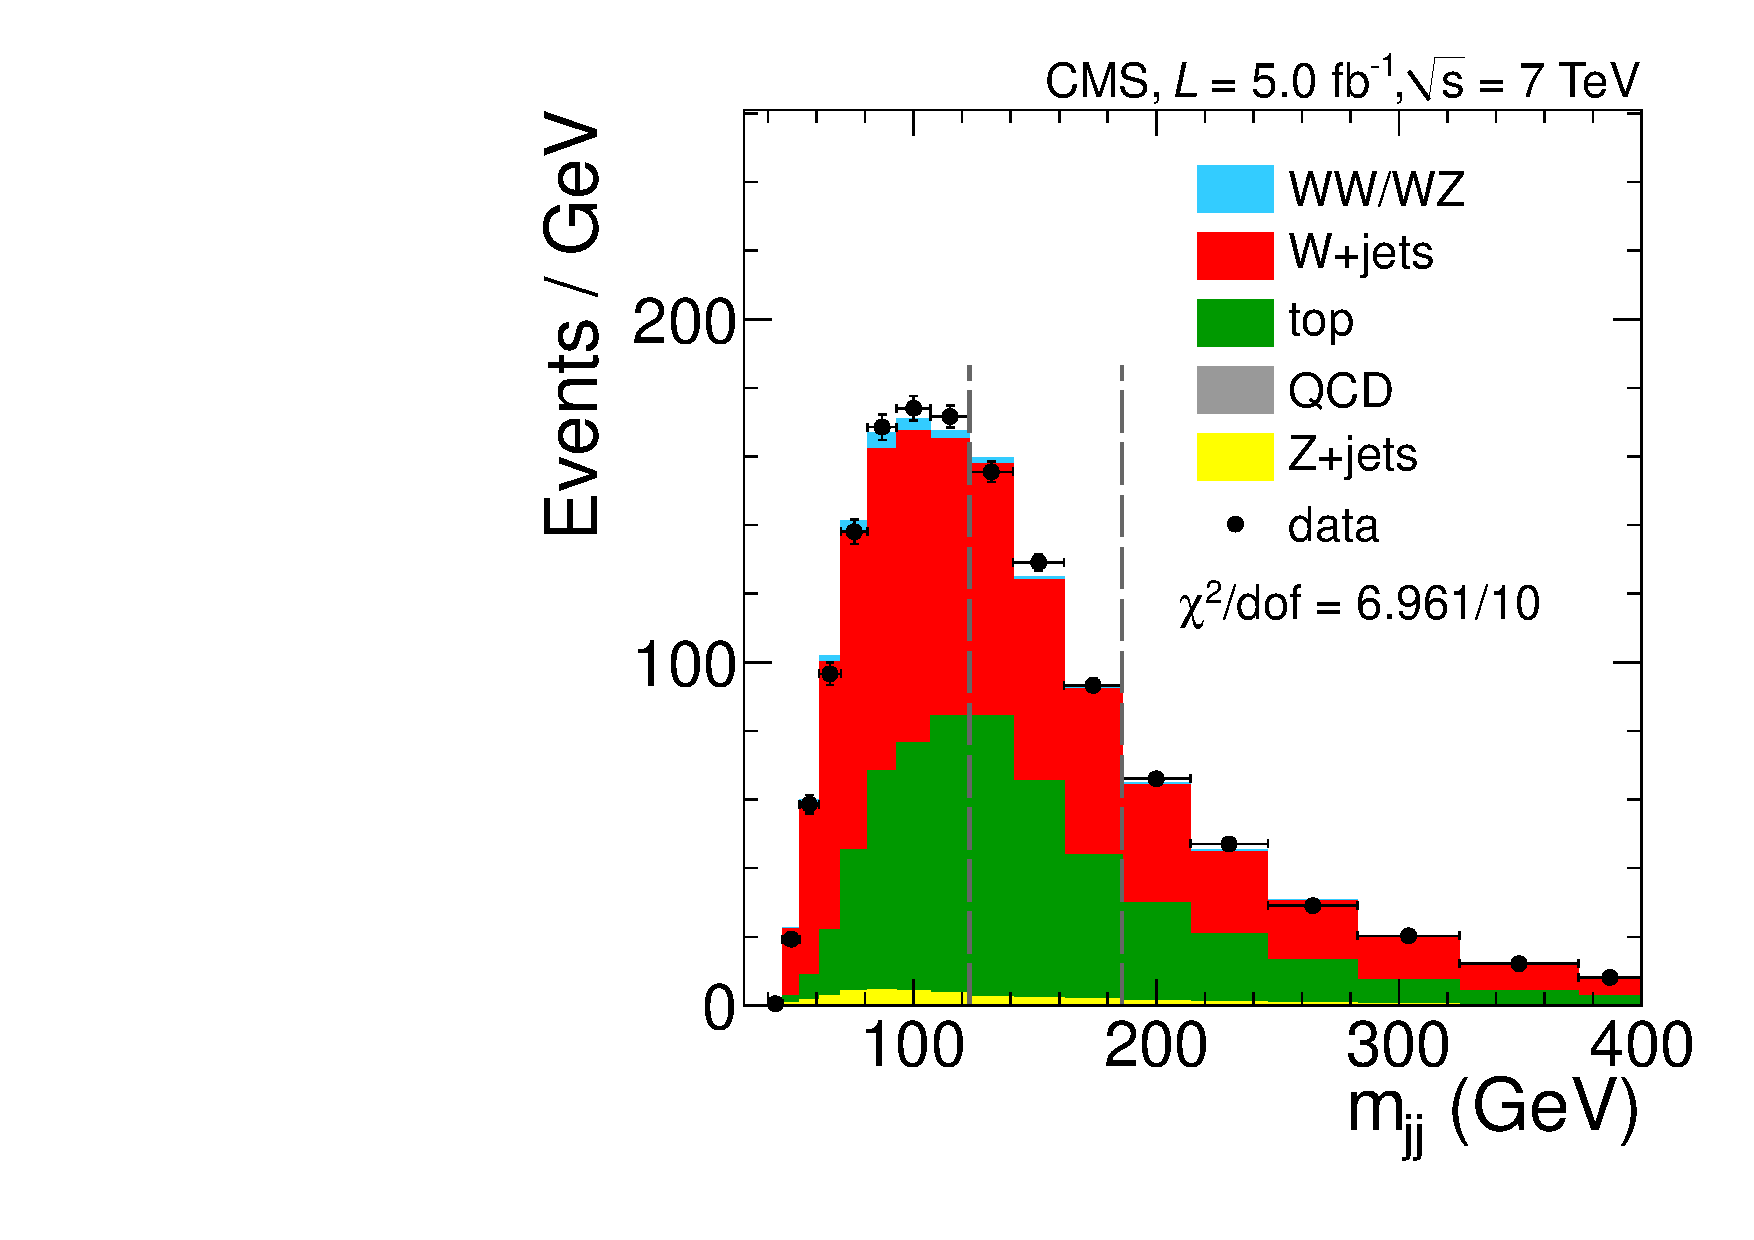
\includegraphics[width=0.49\textwidth]{figs/Wjj_Mjj_Muon_3jets_Stacked.pdf}
   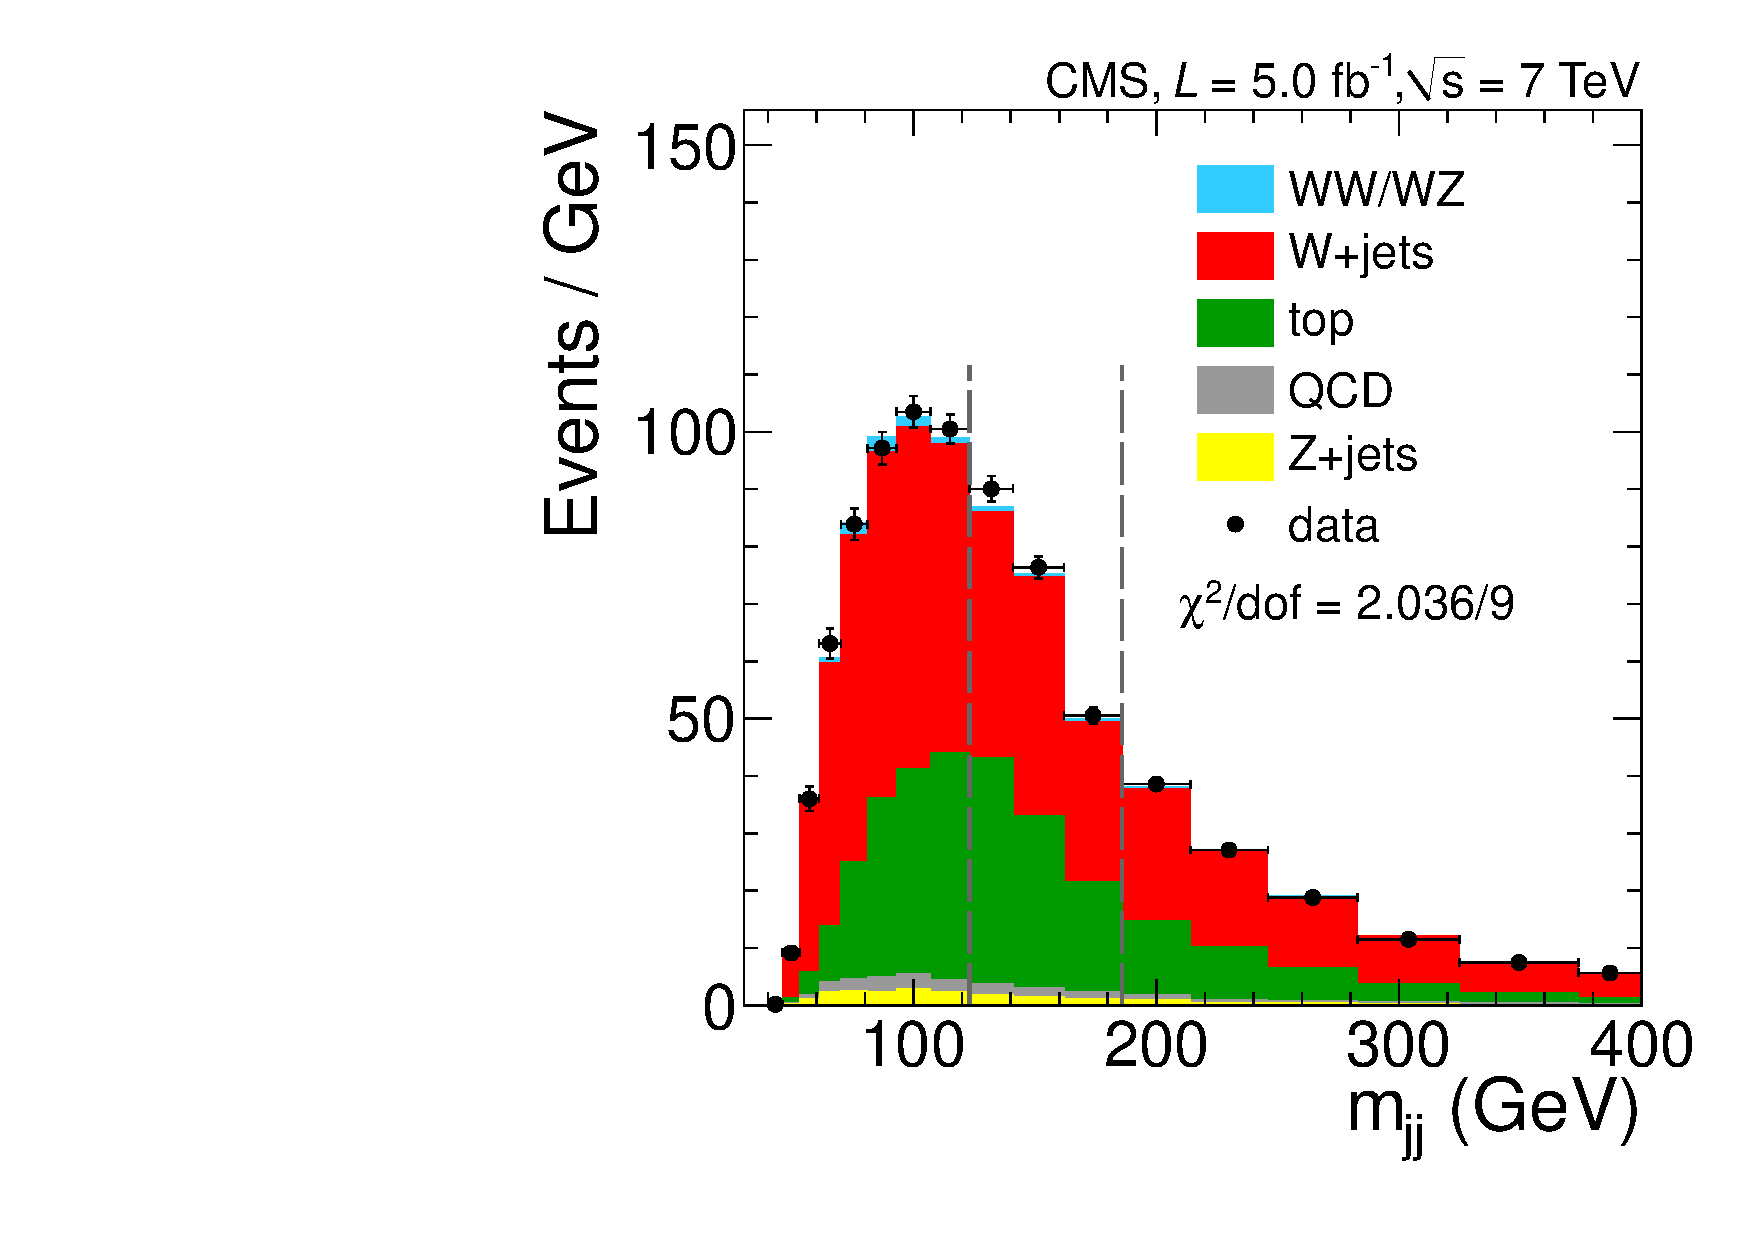
\includegraphics[width=0.49\textwidth]{figs/Wjj_Mjj_Electron_3jets_Stacked.pdf}
   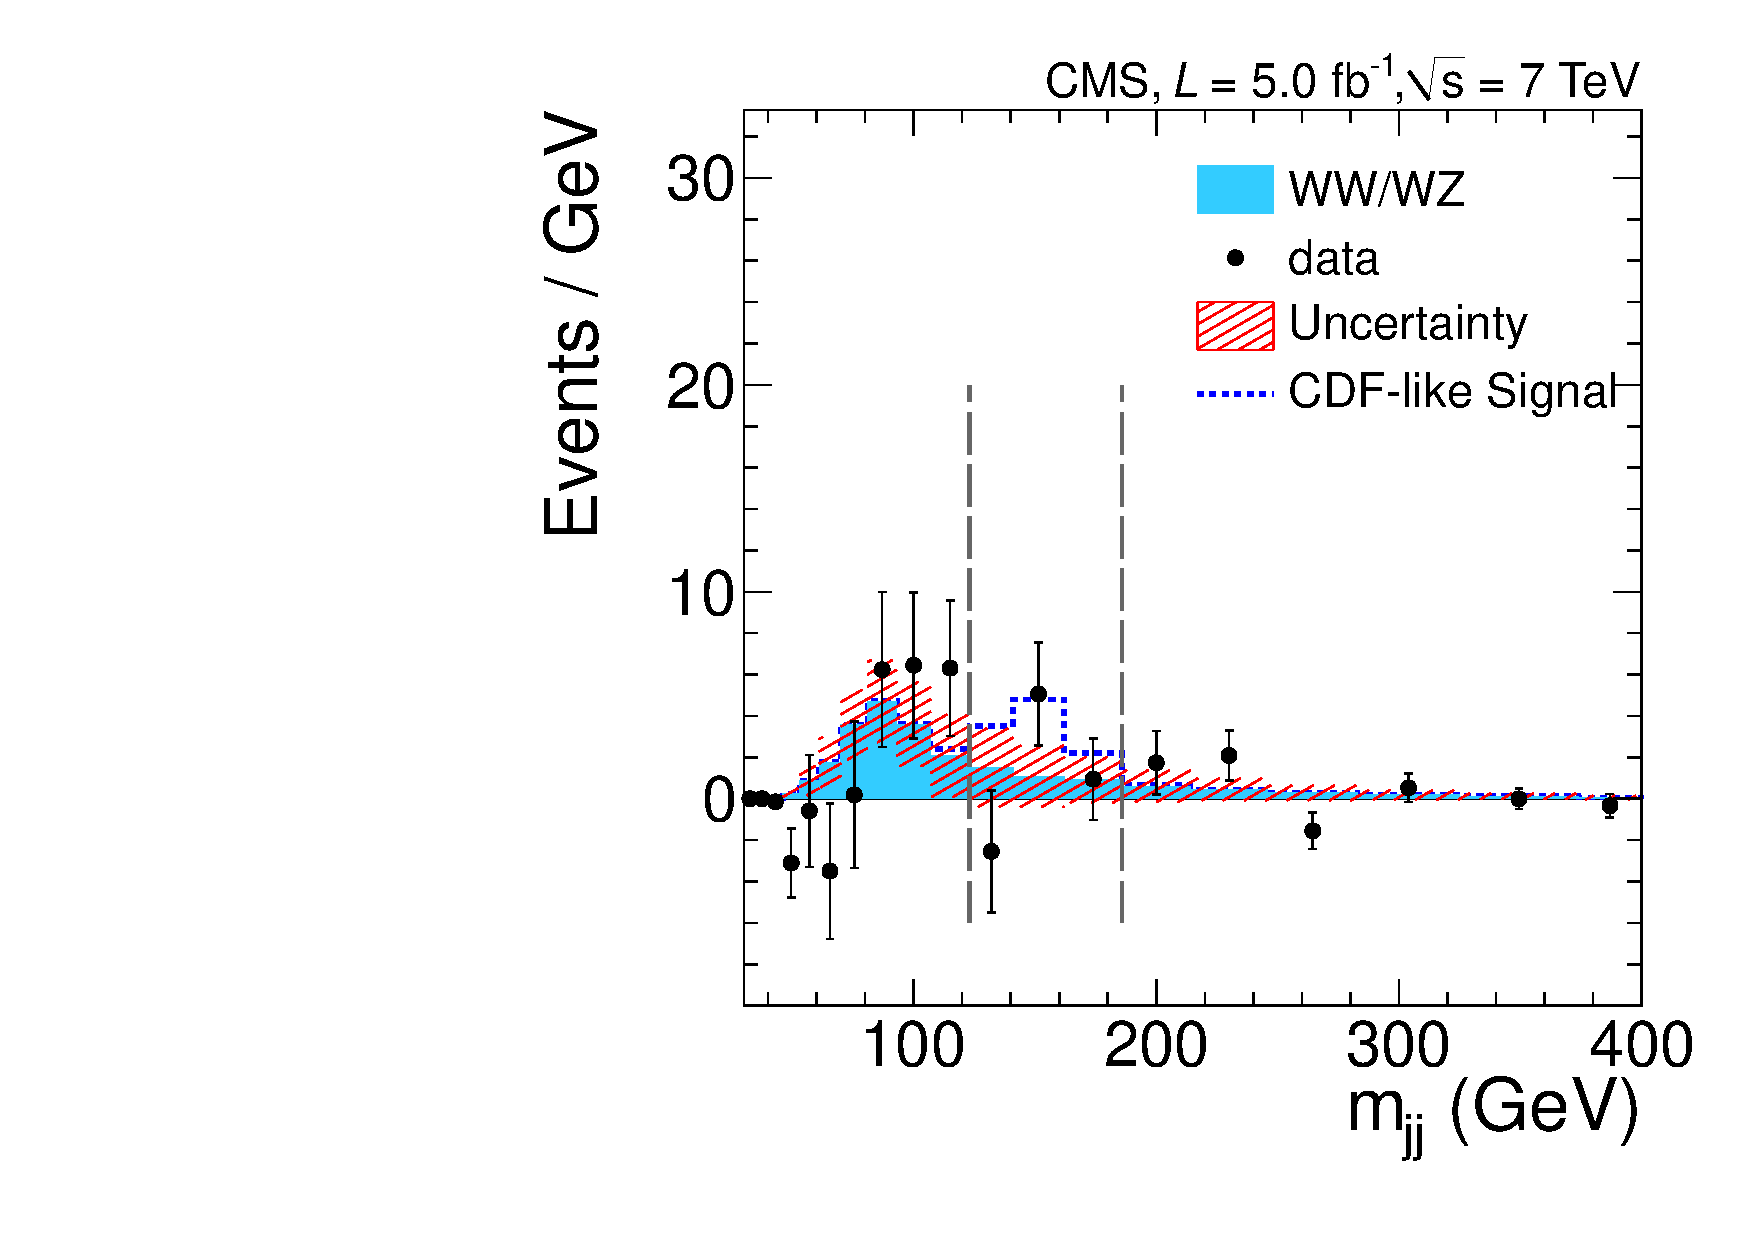
\includegraphics[width=0.49\textwidth]{figs/Wjj_Mjj_Muon_3jets_Subtracted.pdf}
   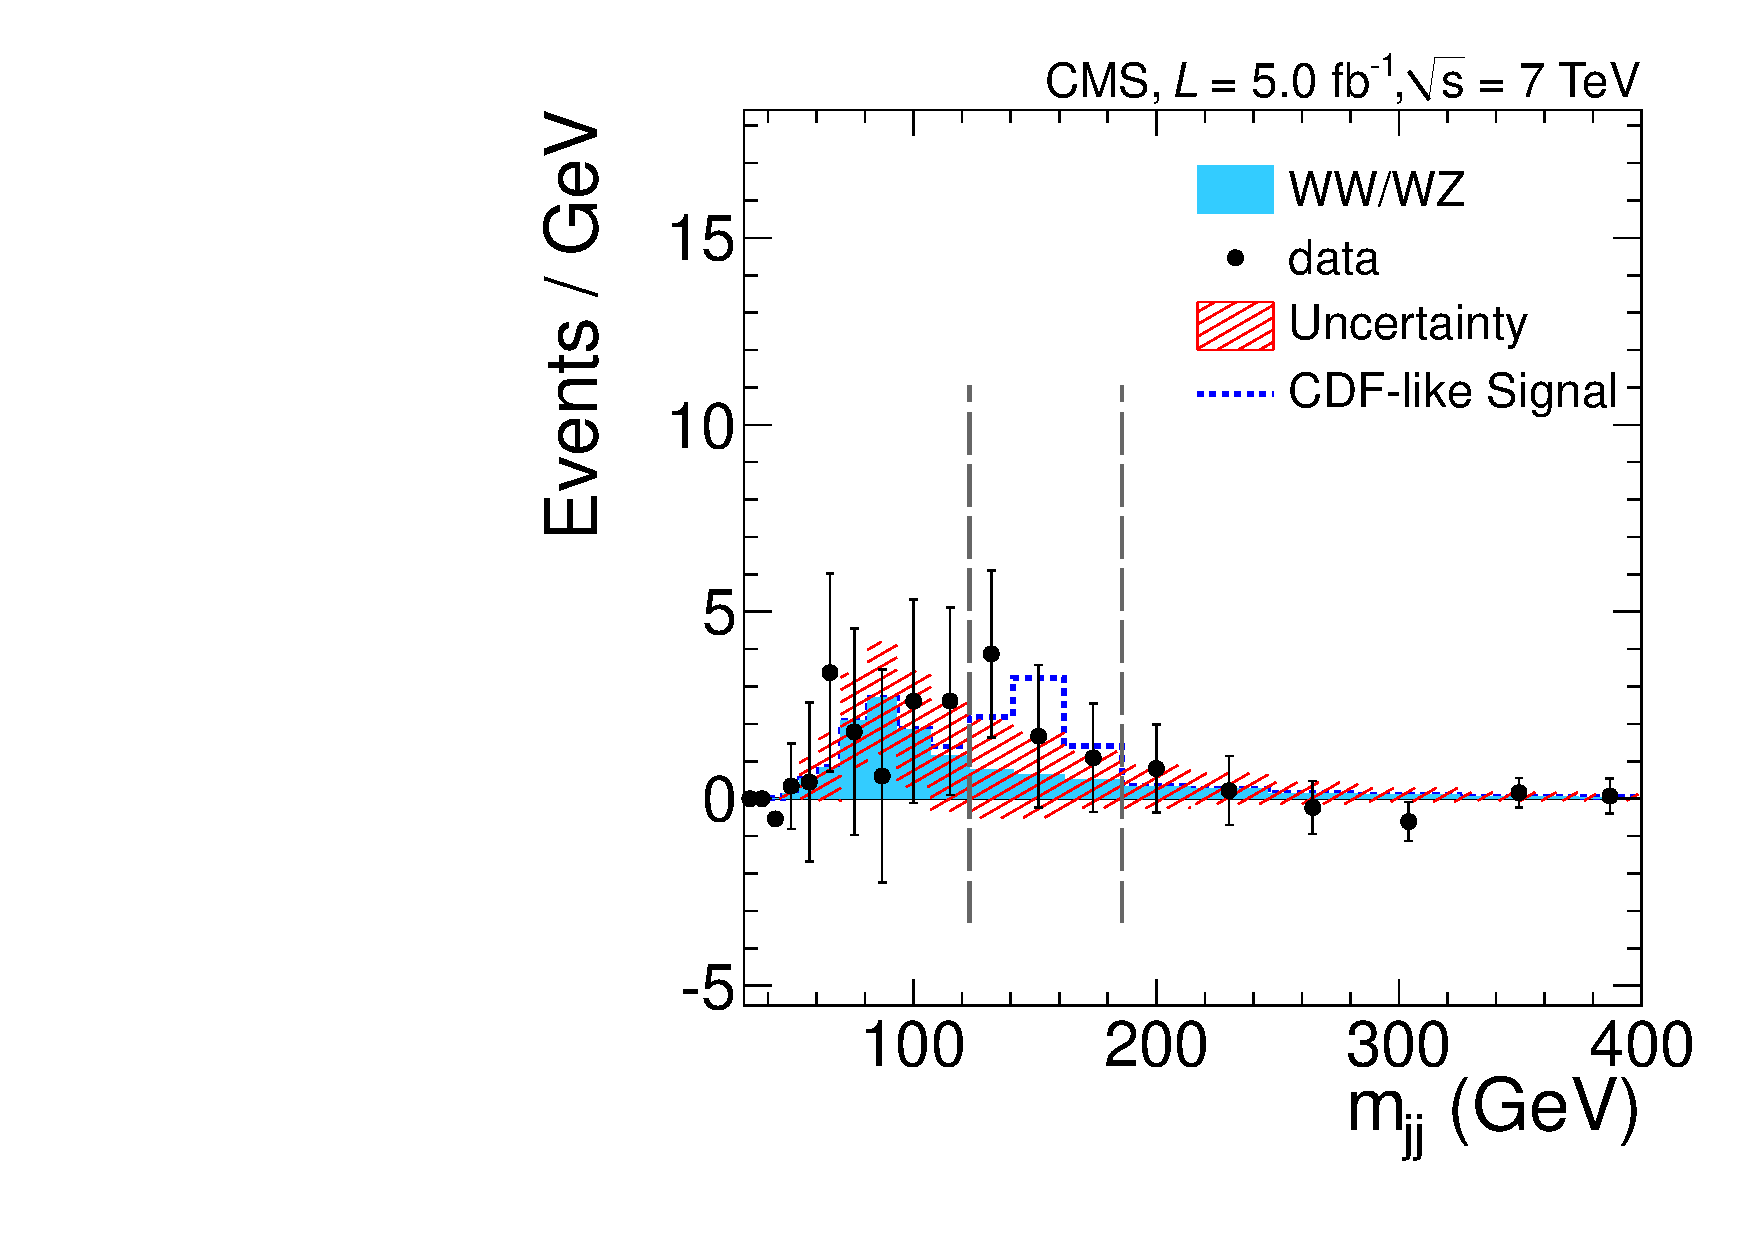
\includegraphics[width=0.49\textwidth]{figs/Wjj_Mjj_Electron_3jets_Subtracted.pdf}
     \caption{(upper row) Distribution of the invariant mass spectrum
       of the leading two jets observed in data in muon plus 3 jets
       (left) and electron plus 3 jets (right) categories.  Overlaid
       are the template distributions used in the likelihood fit to
       the measured \mjj distibution, with their relative
       normalization as obtained from the fit.  The region between the
       vertical dotted lines is excluded in the fit.  Depicted is the
       number of events per GeV, \textit{i.e.}, the raw event count
       can be obtained by multiplying with the bin width.  (lower row)
       The same distribution after subtraction of all SM components
       except the electroweak diboson WW/WZ.  Error bars correspond to
       the statistical uncertainty.  The band represents the
       systematic uncertainty in the sum of the SM components.  }
 \end{figure*}




 \begin{figure*}[h!t]
   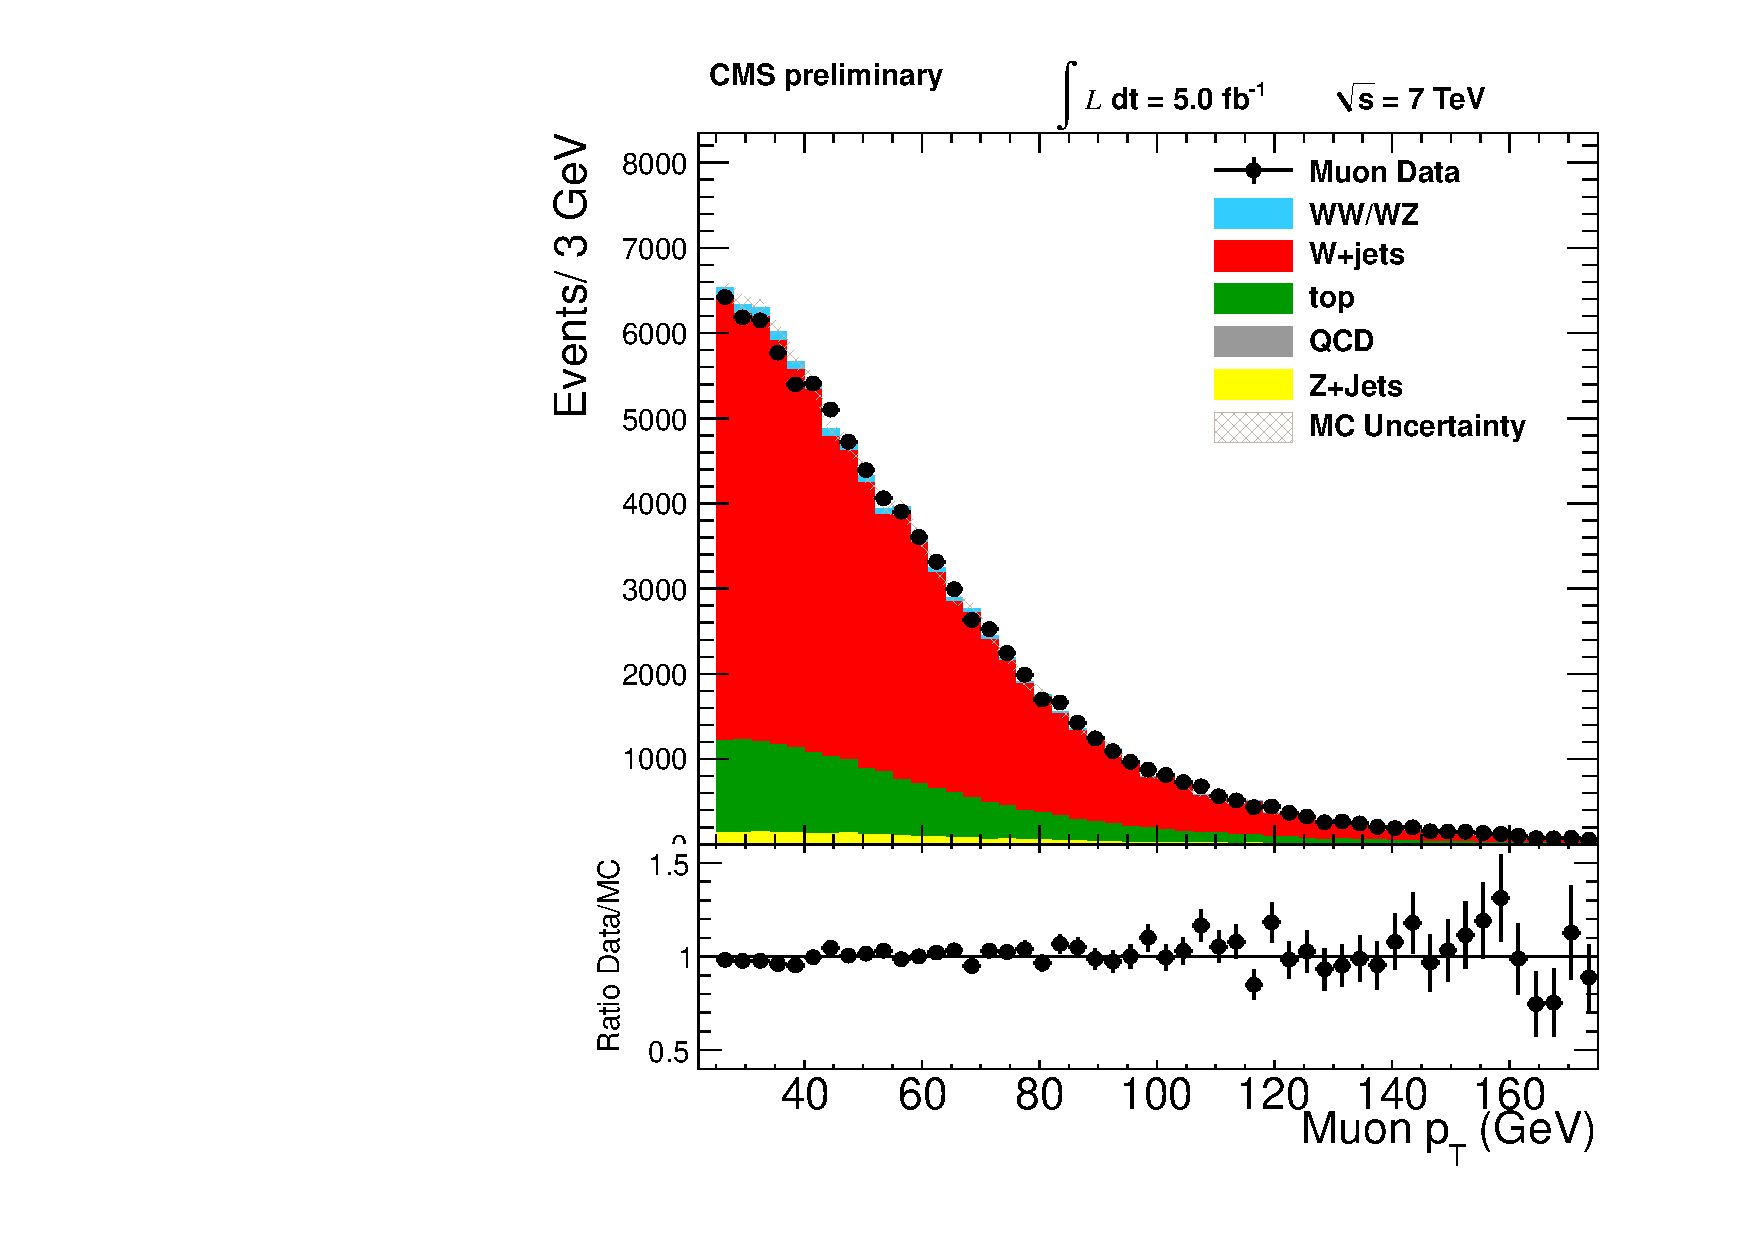
\includegraphics[width=0.3\textwidth]{figs/mu_W_muon_pt.pdf}
   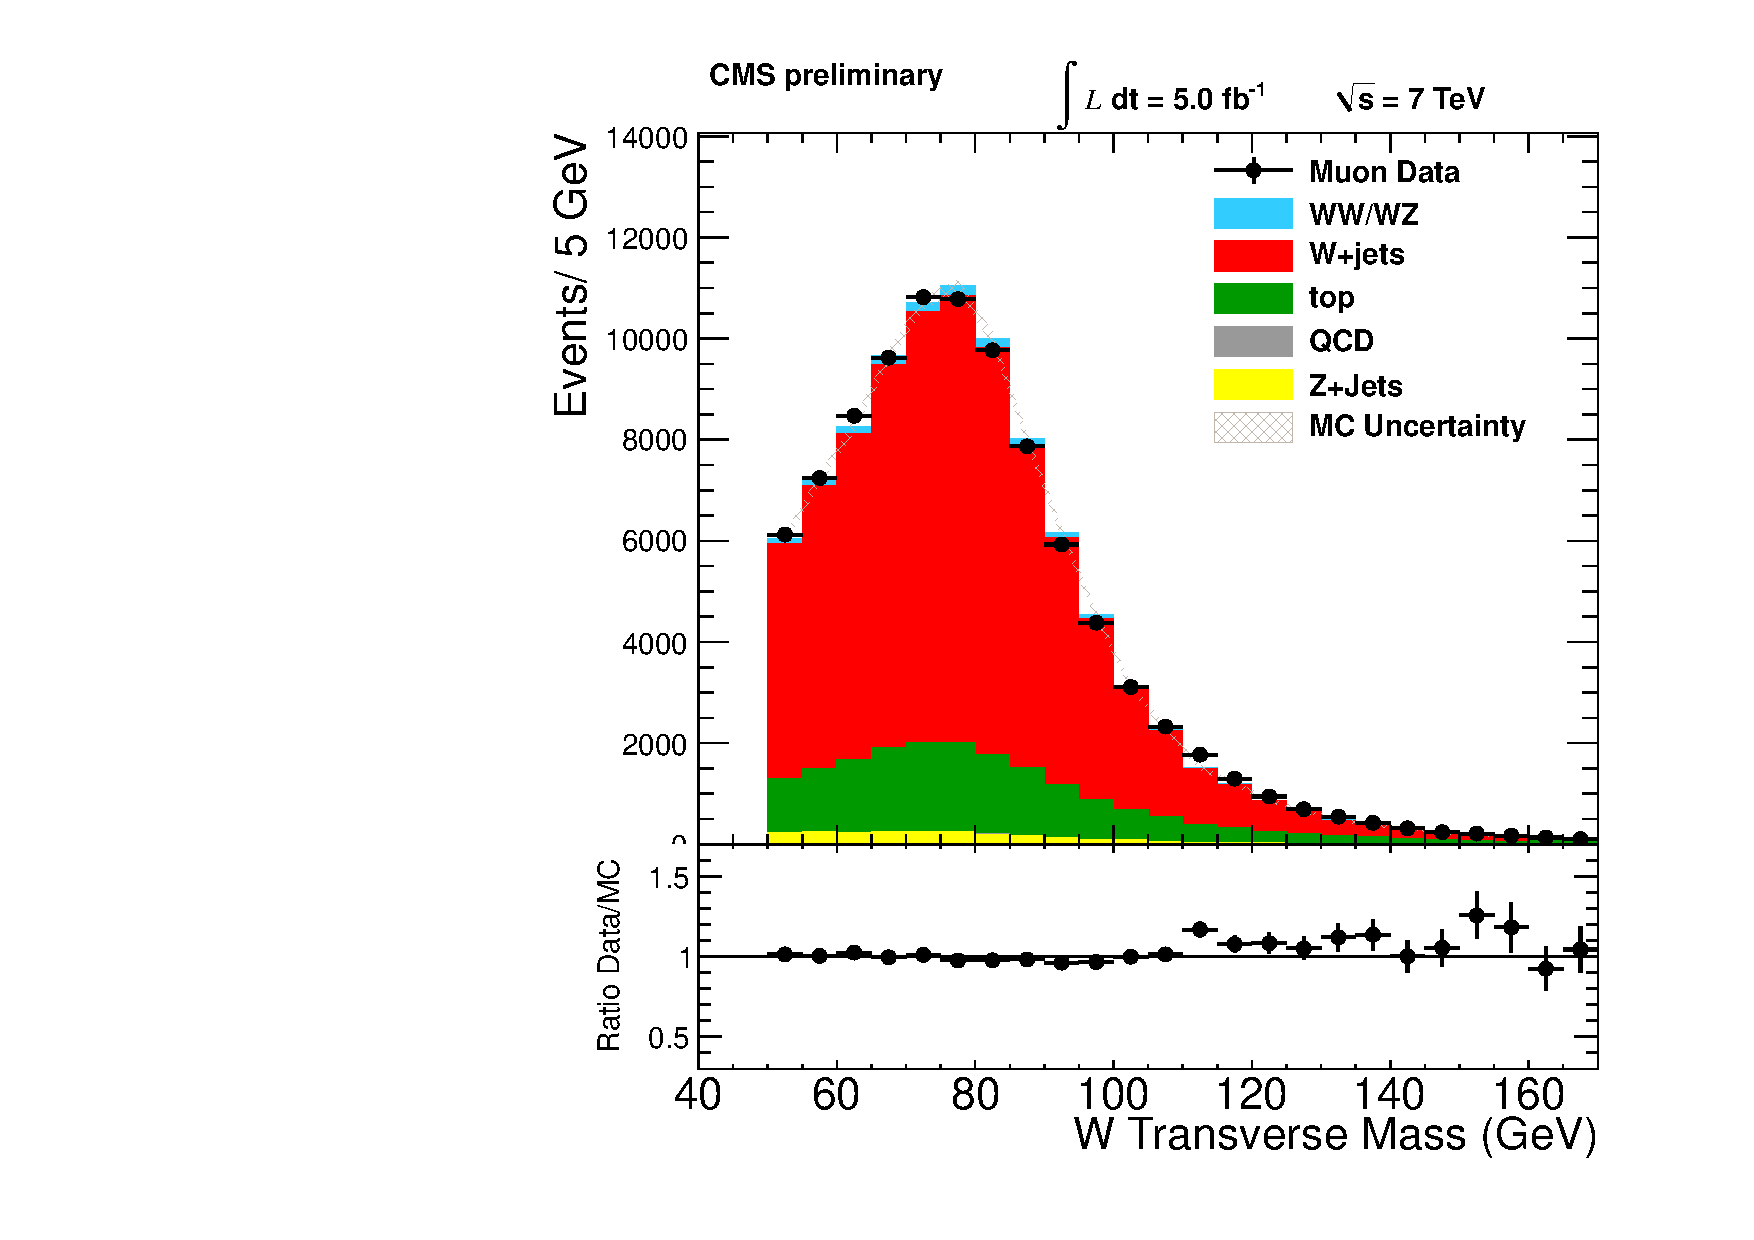
\includegraphics[width=0.3\textwidth]{figs/mu_W_mt.pdf}
   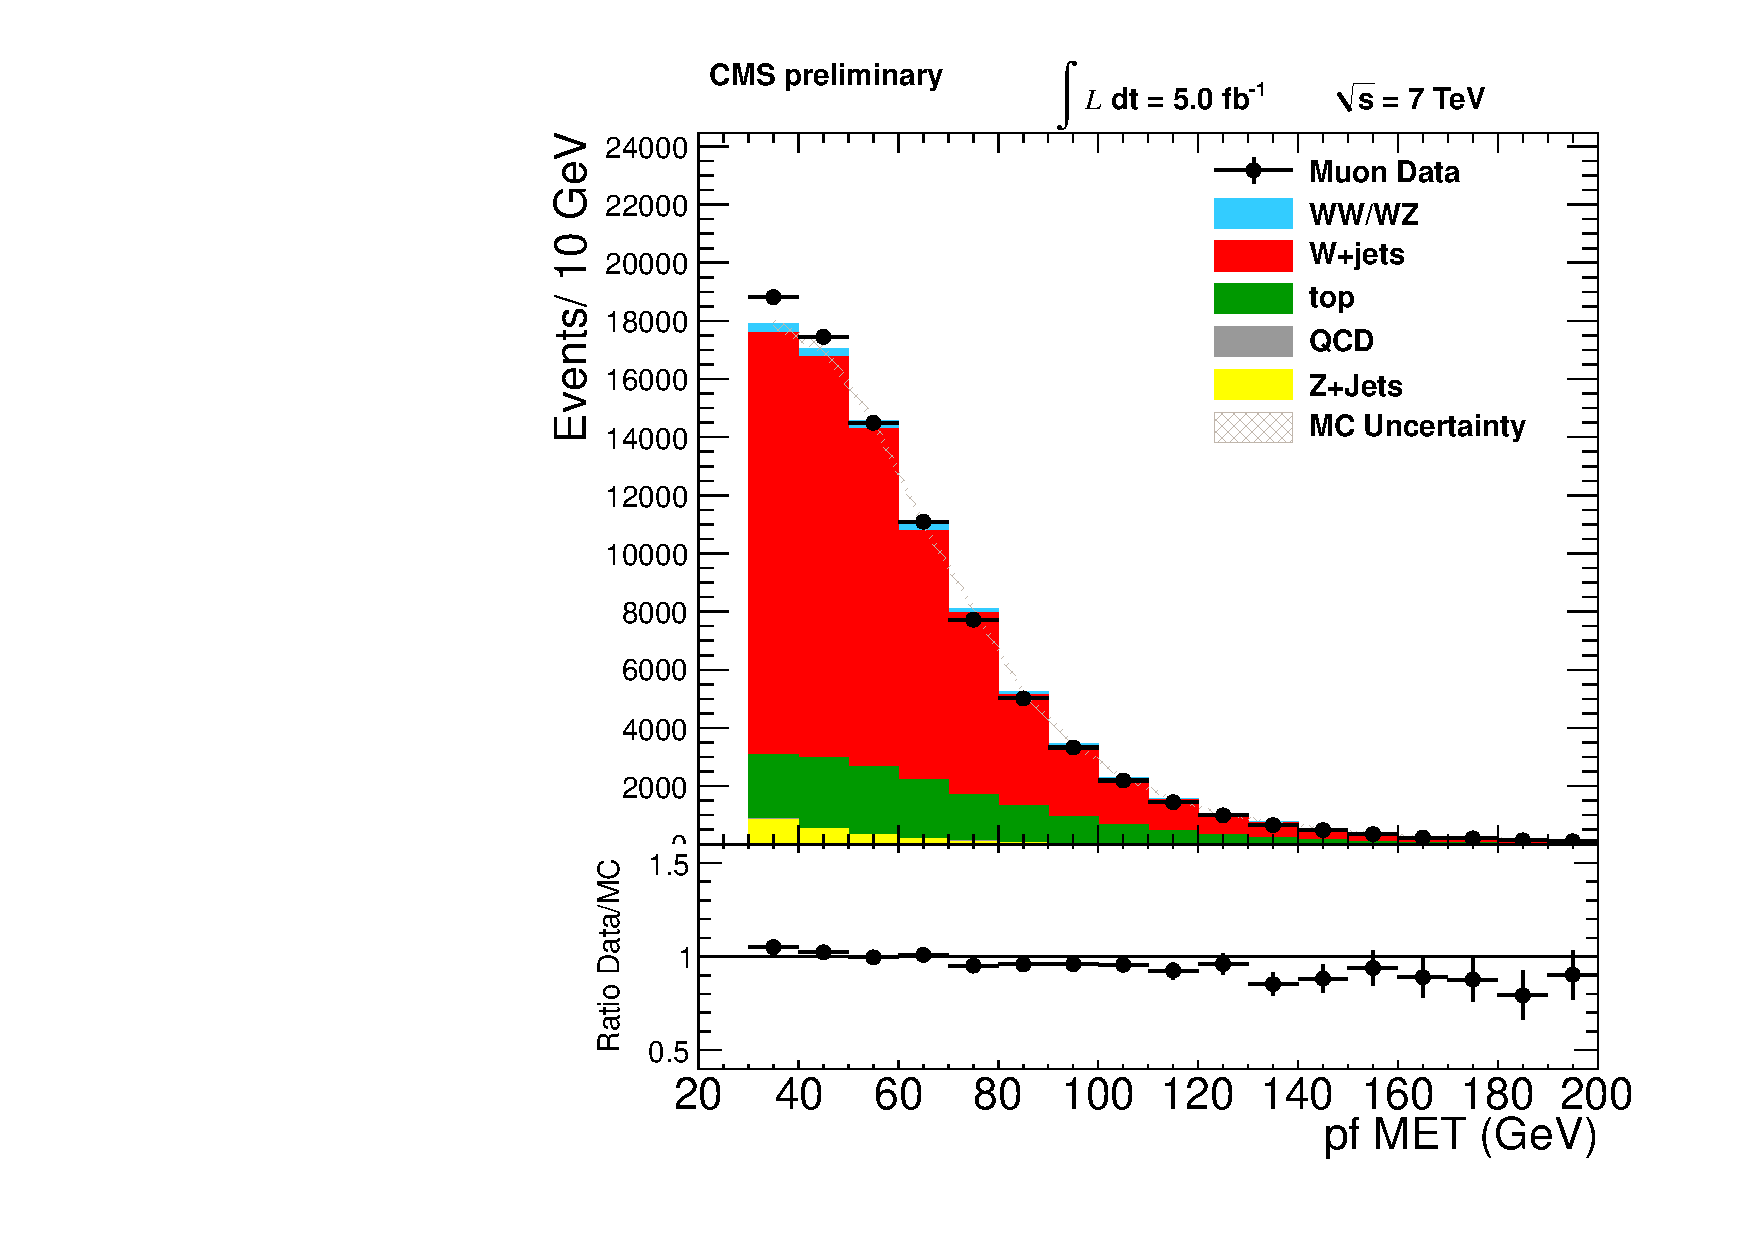
\includegraphics[width=0.3\textwidth]{figs/mu_event_met_pfmet.pdf}
   \caption{Comparison of the distributions in data and MC for the
     muon plus jets event sample after event selection (left) of the
     transverse momentum of the muon candidate, (middle) of the
     transverse momentum of the reconstructed W candidate, (right) of
     the missing transverse energy. The error bars on the data points
     are statistical only.  The relative normalization of the various
     MC samples are taken from the result of the fit to the \mjj
     spectrum.  }
 \end{figure*}


 \begin{figure*}[h!t]
   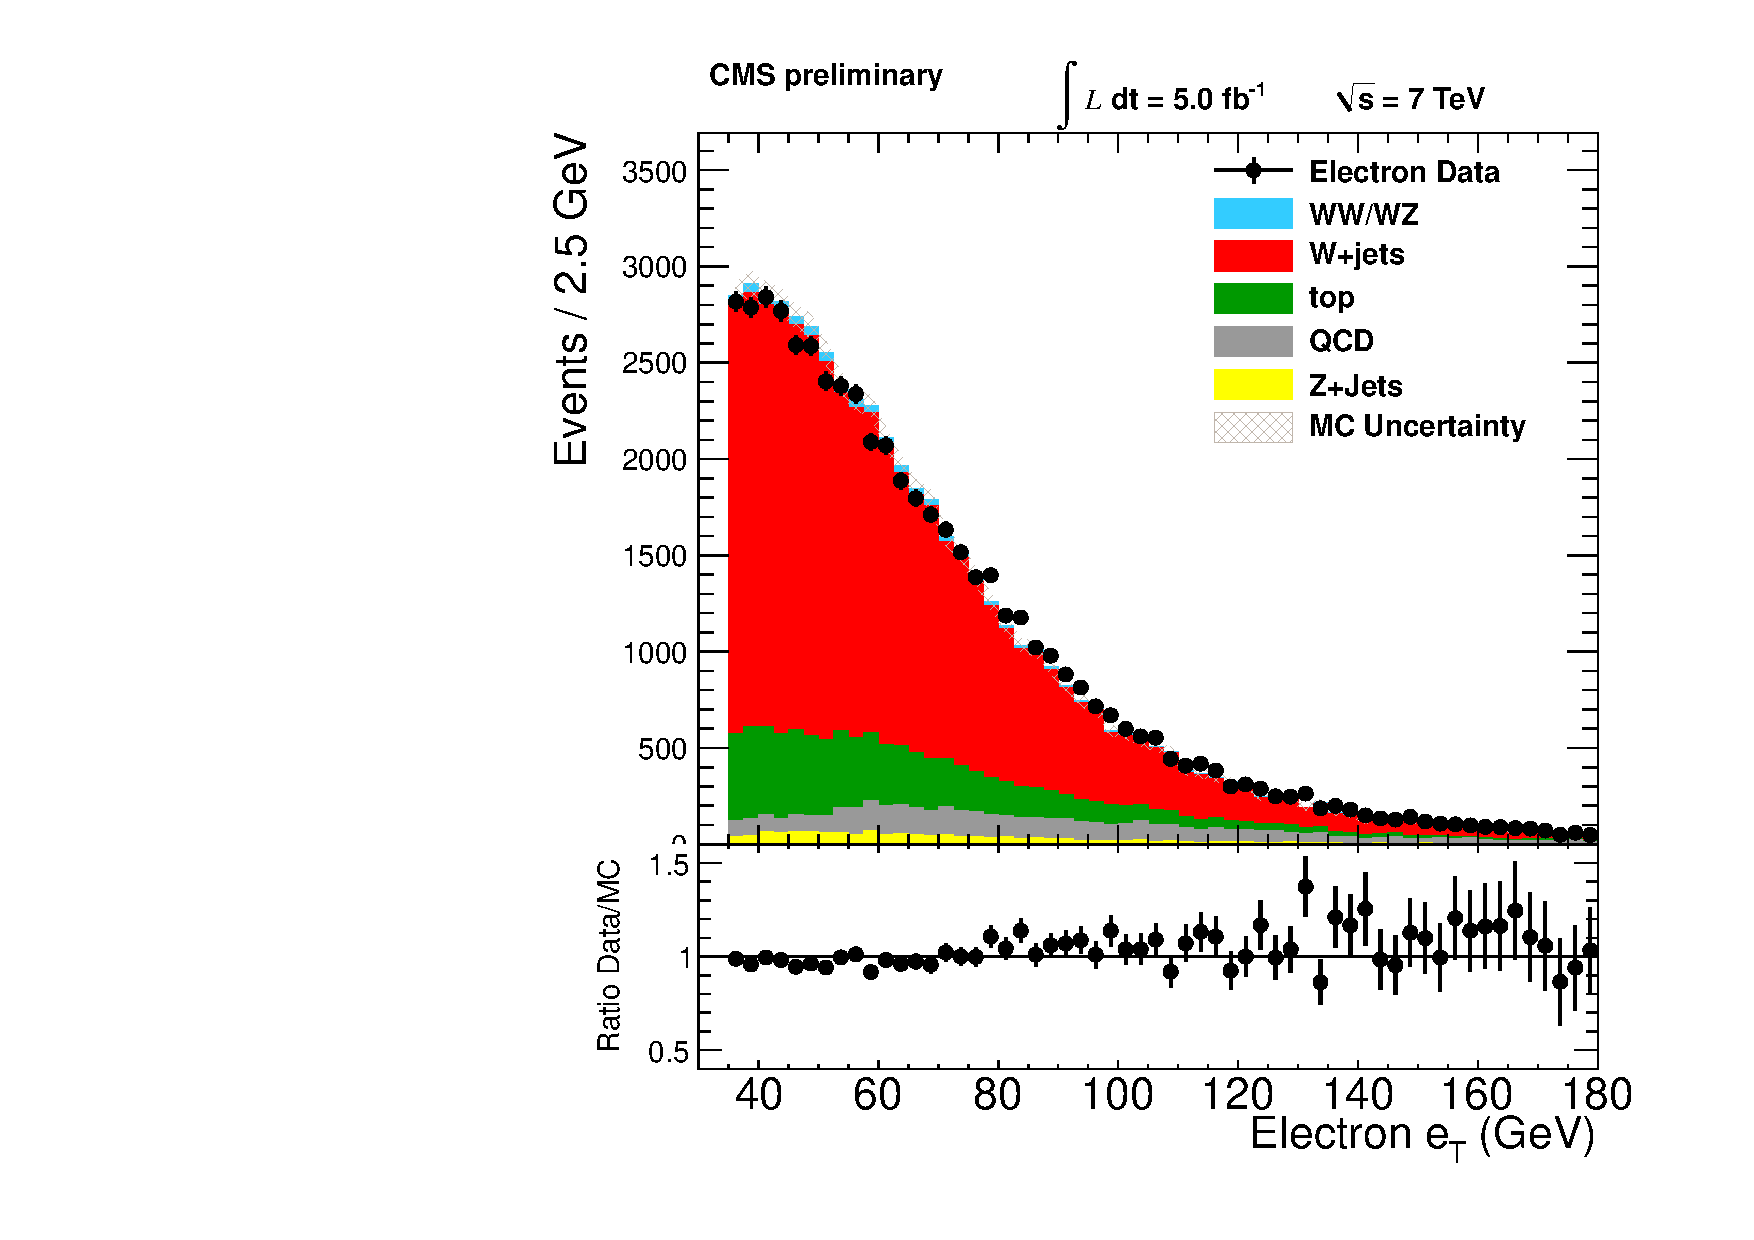
\includegraphics[width=0.3\textwidth]{figs/elec_W_electron_et.pdf}
   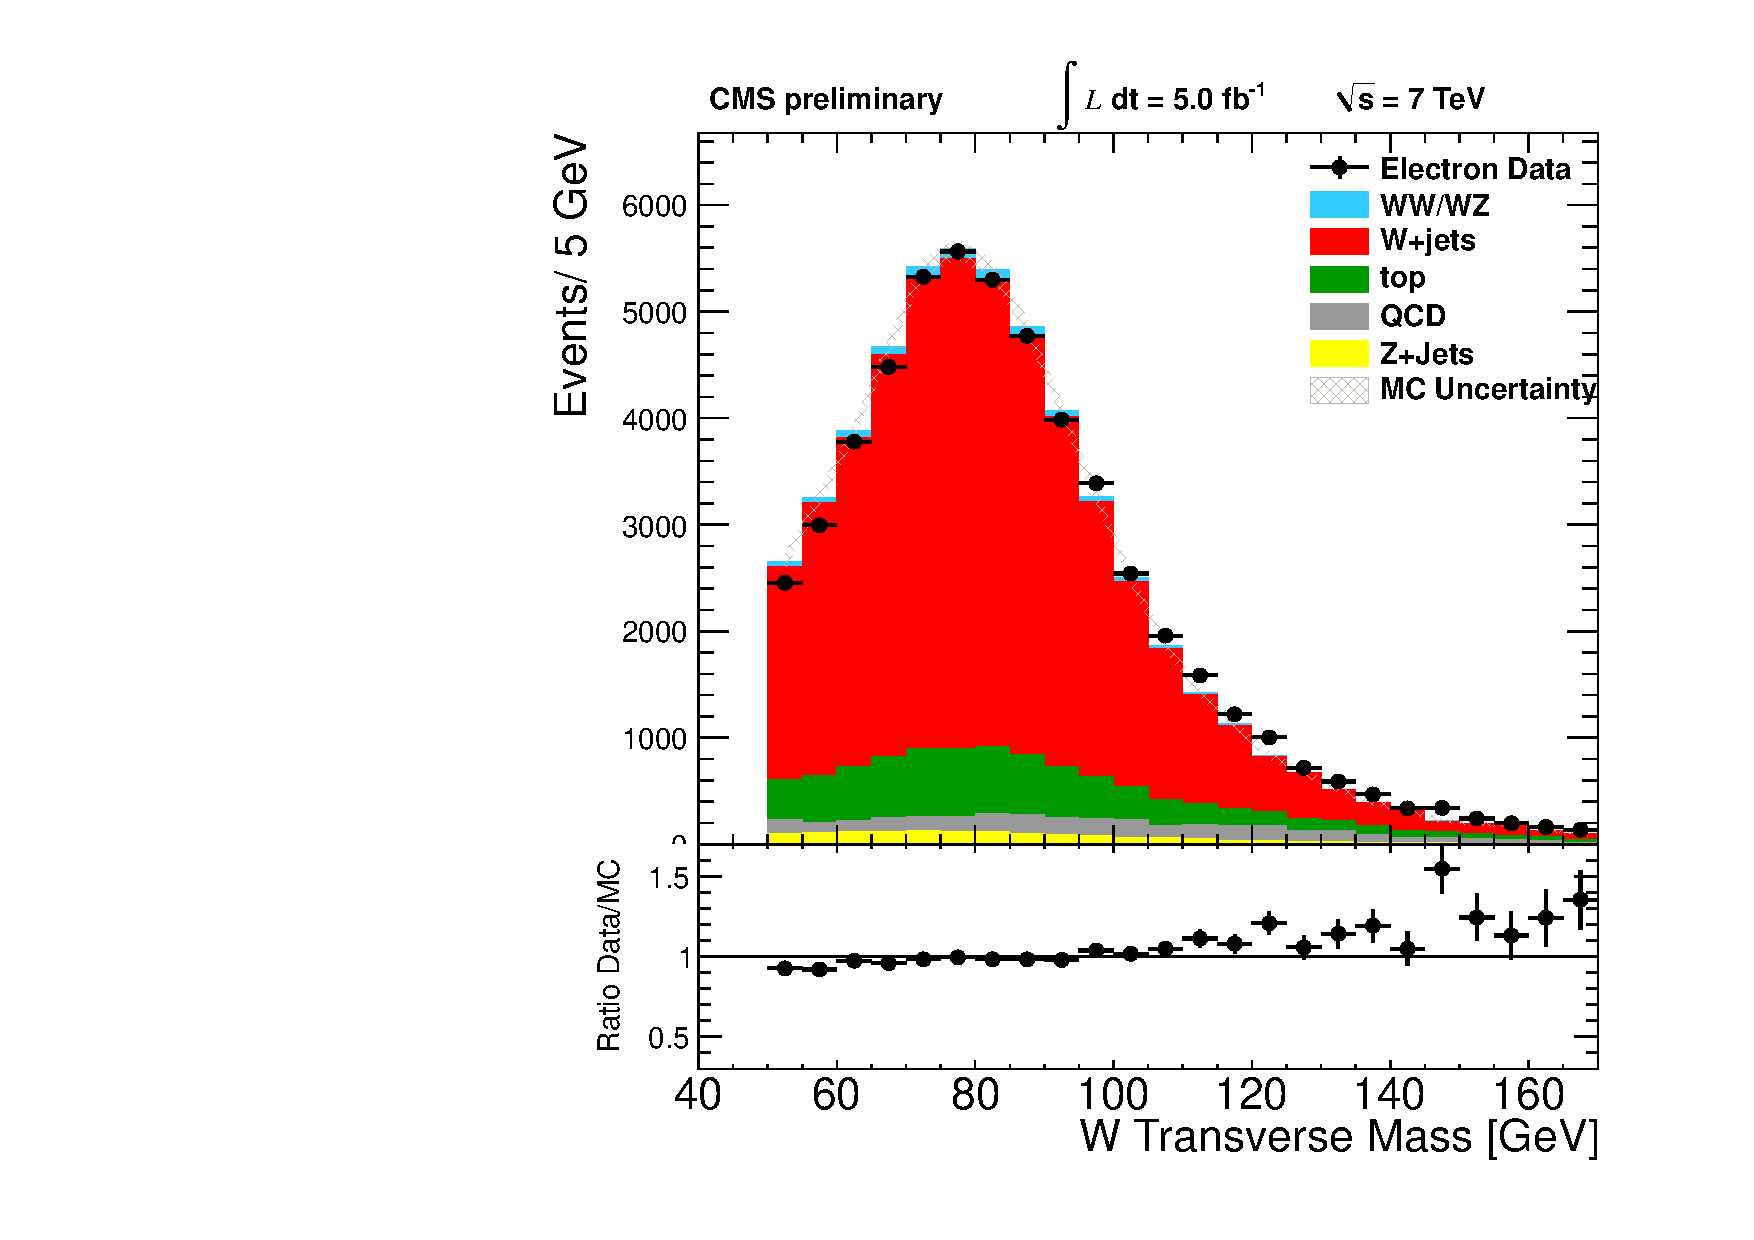
\includegraphics[width=0.3\textwidth]{figs/el_W_mt.pdf}
   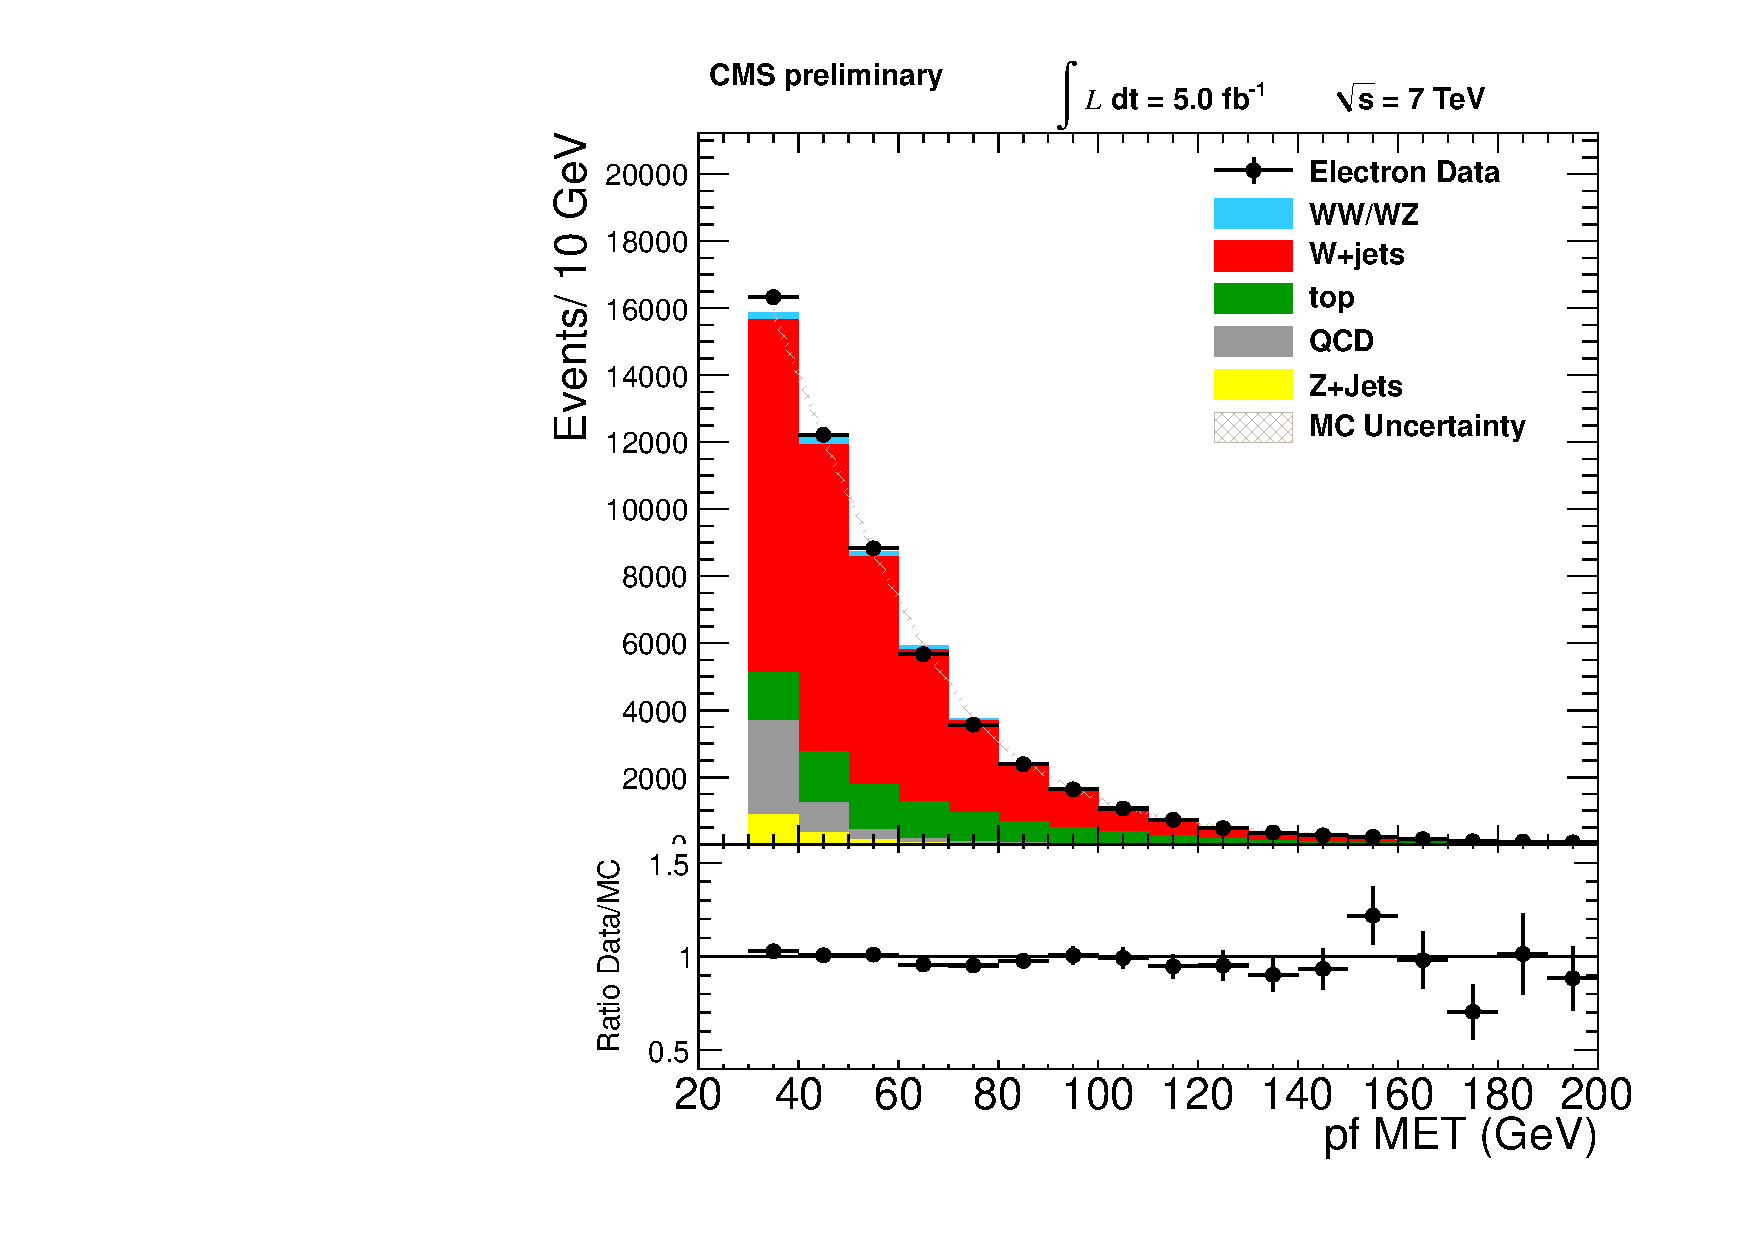
\includegraphics[width=0.3\textwidth]{figs/el_event_met_pfmet.pdf}
   \caption{Comparison of the distributions in data and MC for the
     electron plus jets event sample after event selection (left) of
     the transverse energy of the electron candidate, (middle) of the
     transverse momentum of the reconstructed W candidate, (right) of
     the missing transverse energy. The error bars on the data points
     are statistical only.  The relative normalization of the various
     MC samples are taken from the result of the fit to the \mjj
     spectrum.  }
 \end{figure*}



 \begin{figure*}[h!t]
   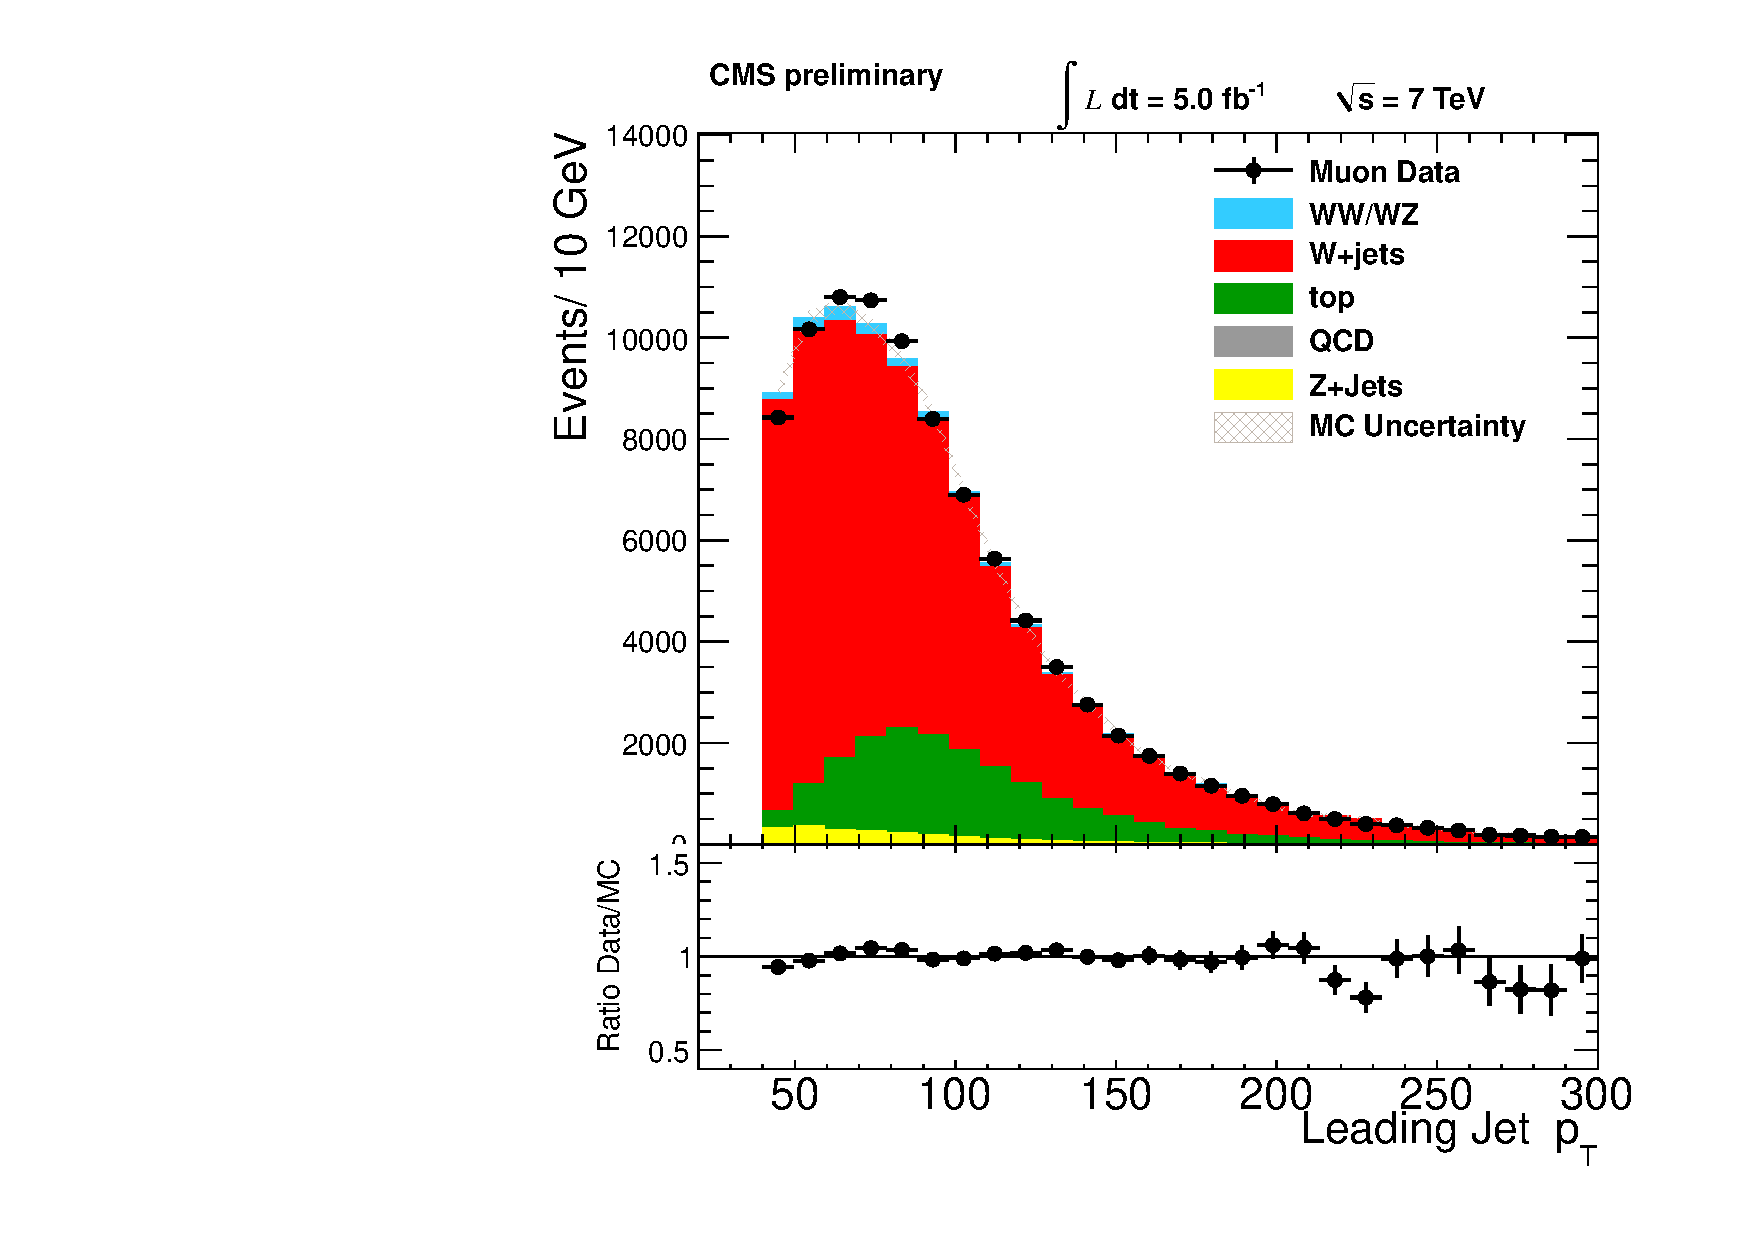
\includegraphics[width=0.49\textwidth]{figs/mu_jetld_pt.pdf}
   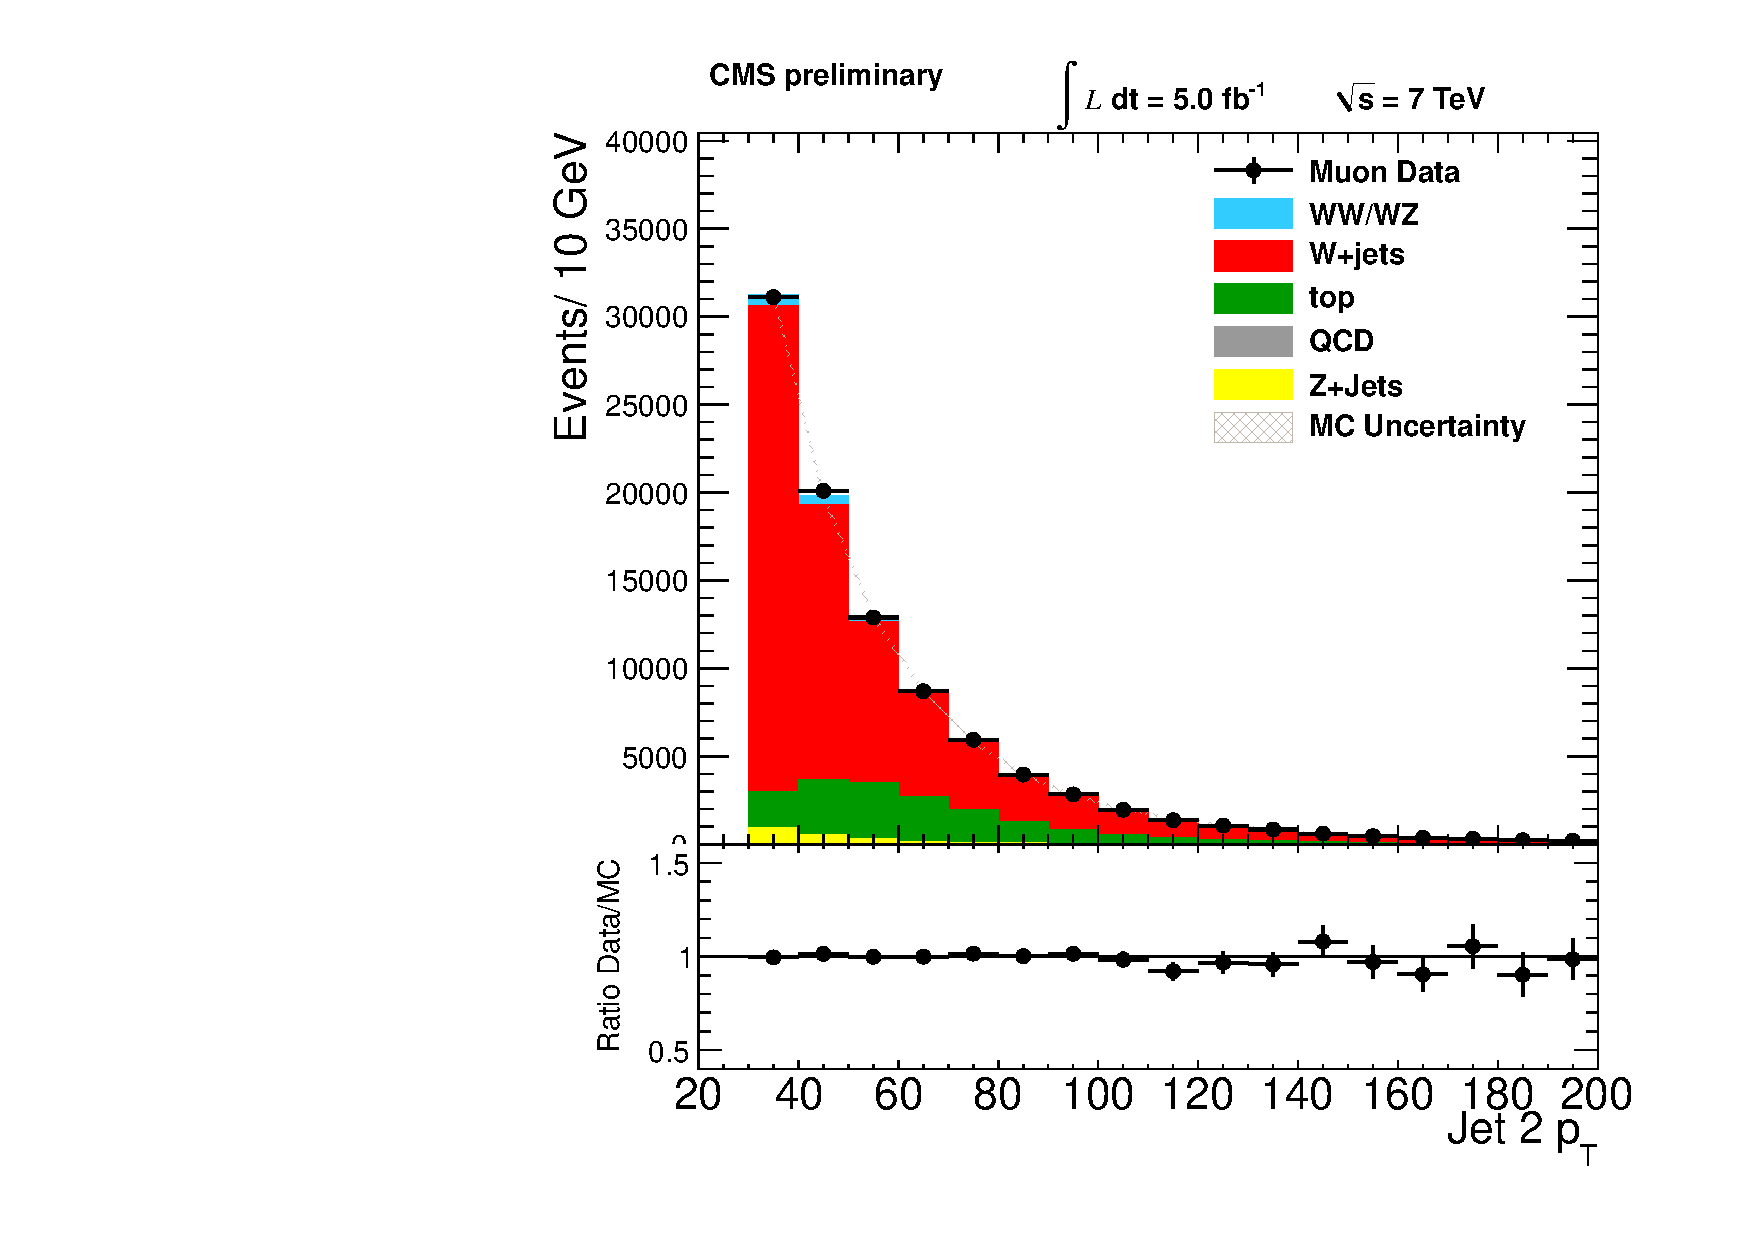
\includegraphics[width=0.49\textwidth]{figs/mu_jetnt_pt.pdf}
   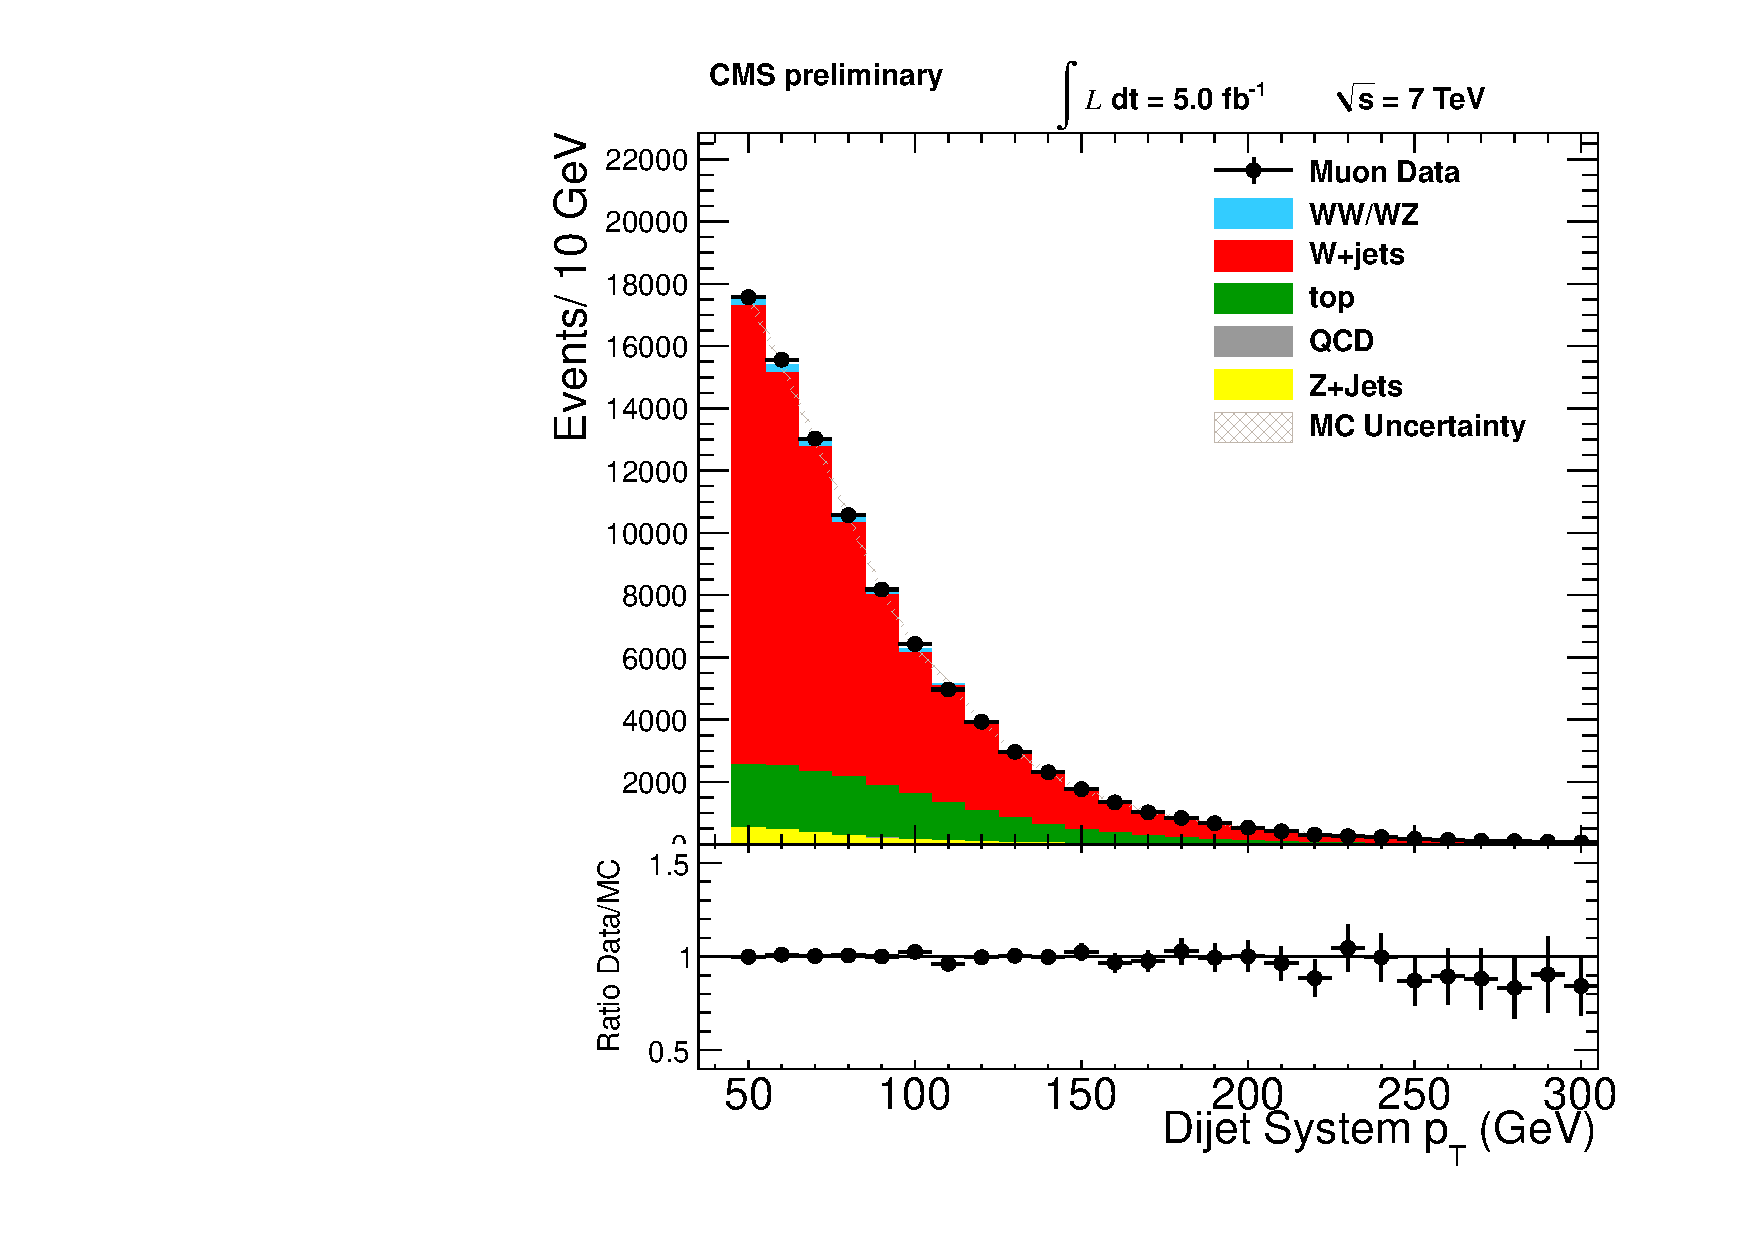
\includegraphics[width=0.49\textwidth]{figs/mu_dijet_pt.pdf}
   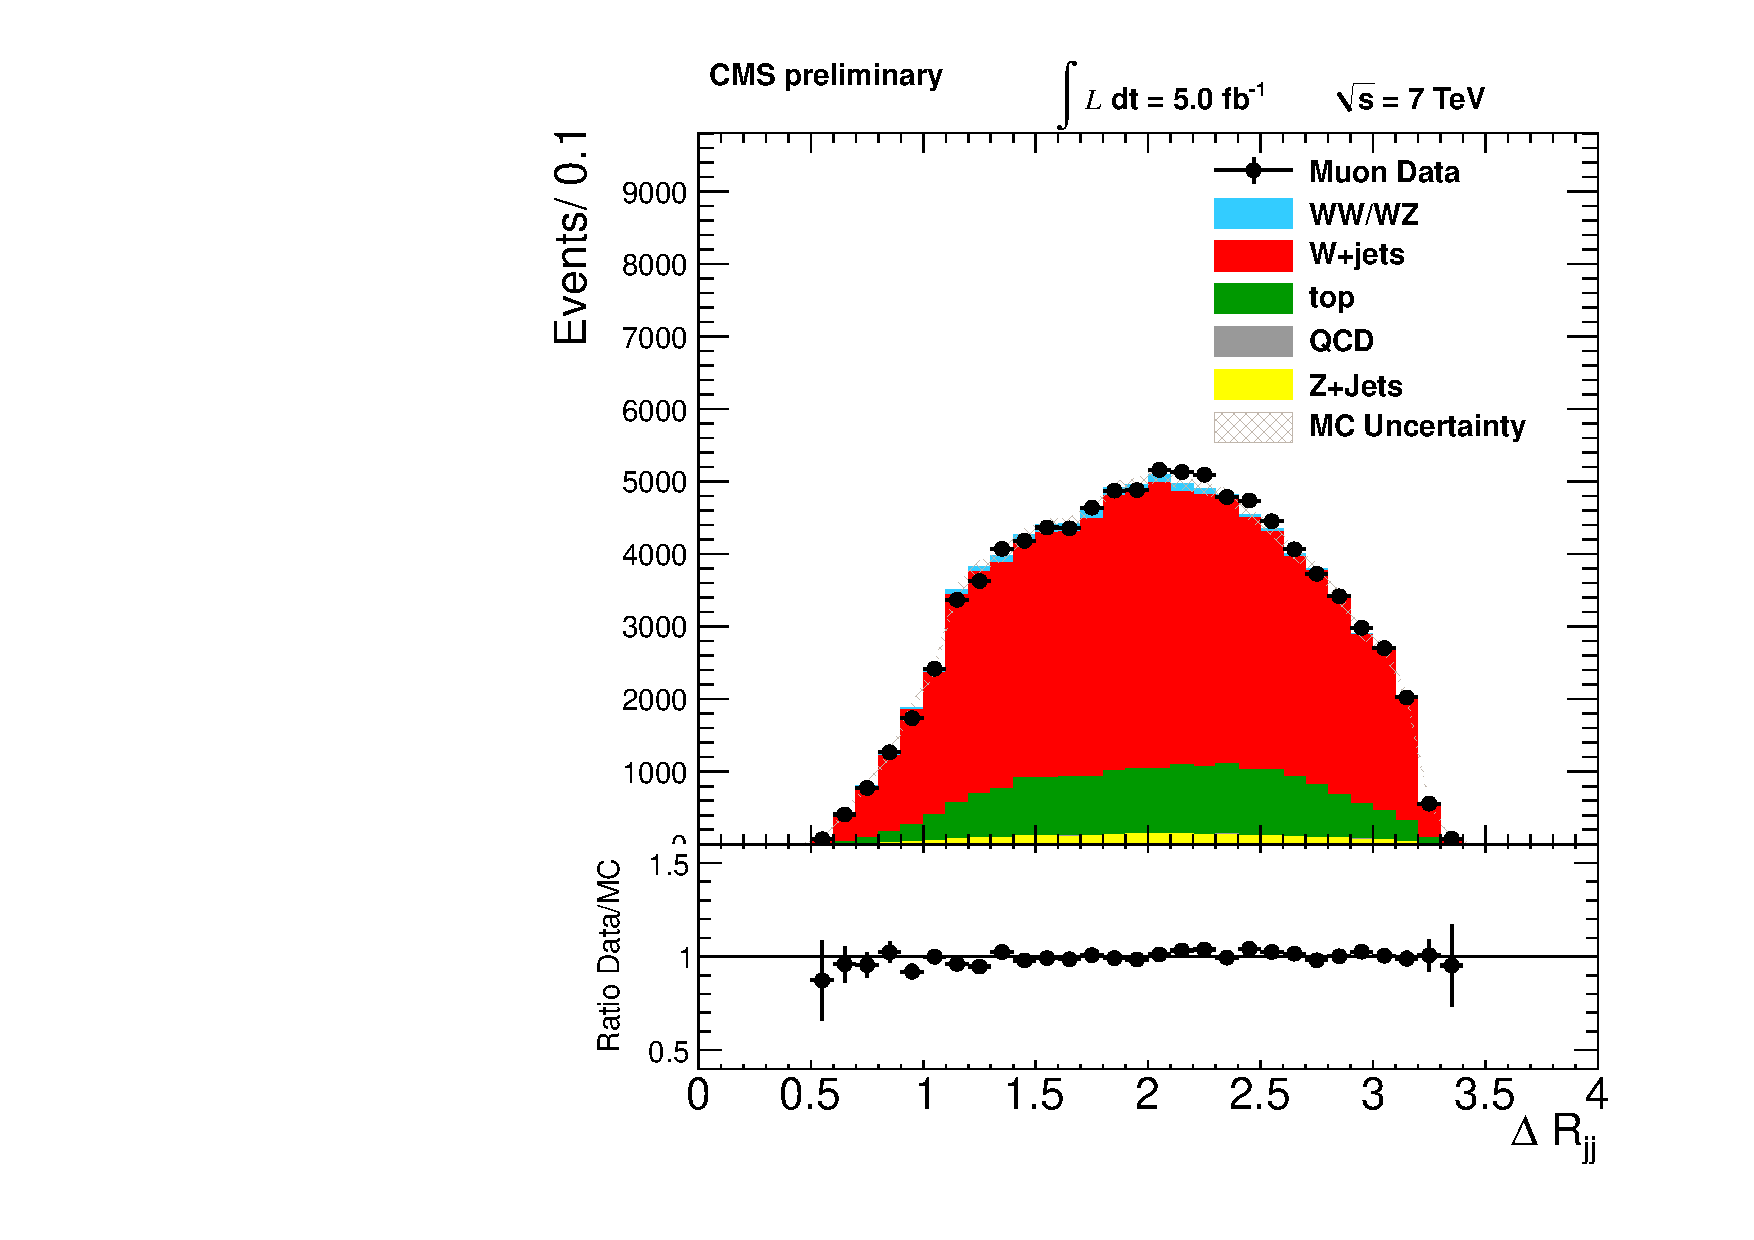
\includegraphics[width=0.49\textwidth]{figs/mu_deltaRjj.pdf}
   \caption{Comparison of the distributions in data and MC for the
     muon plus jets event sample after event selection (upper left) of
     the transverse momentum of the leading jet, (upper right) of the
     transverse momentum of the second leading jet, (lower left) of
     the dijet transverse momentum, (lower right) of the dijet
     distance parameter $\Delta R= \sqrt{(\Delta \eta_{jj})^2 +
       (\Delta \phi_{jj})^2}$. The error bars on the data points are
     statistical only.  The relative normalization of the various MC
     samples are taken from the result of the fit to the \mjj
     spectrum.  }
 \end{figure*}

 \begin{figure*}[h!t]
   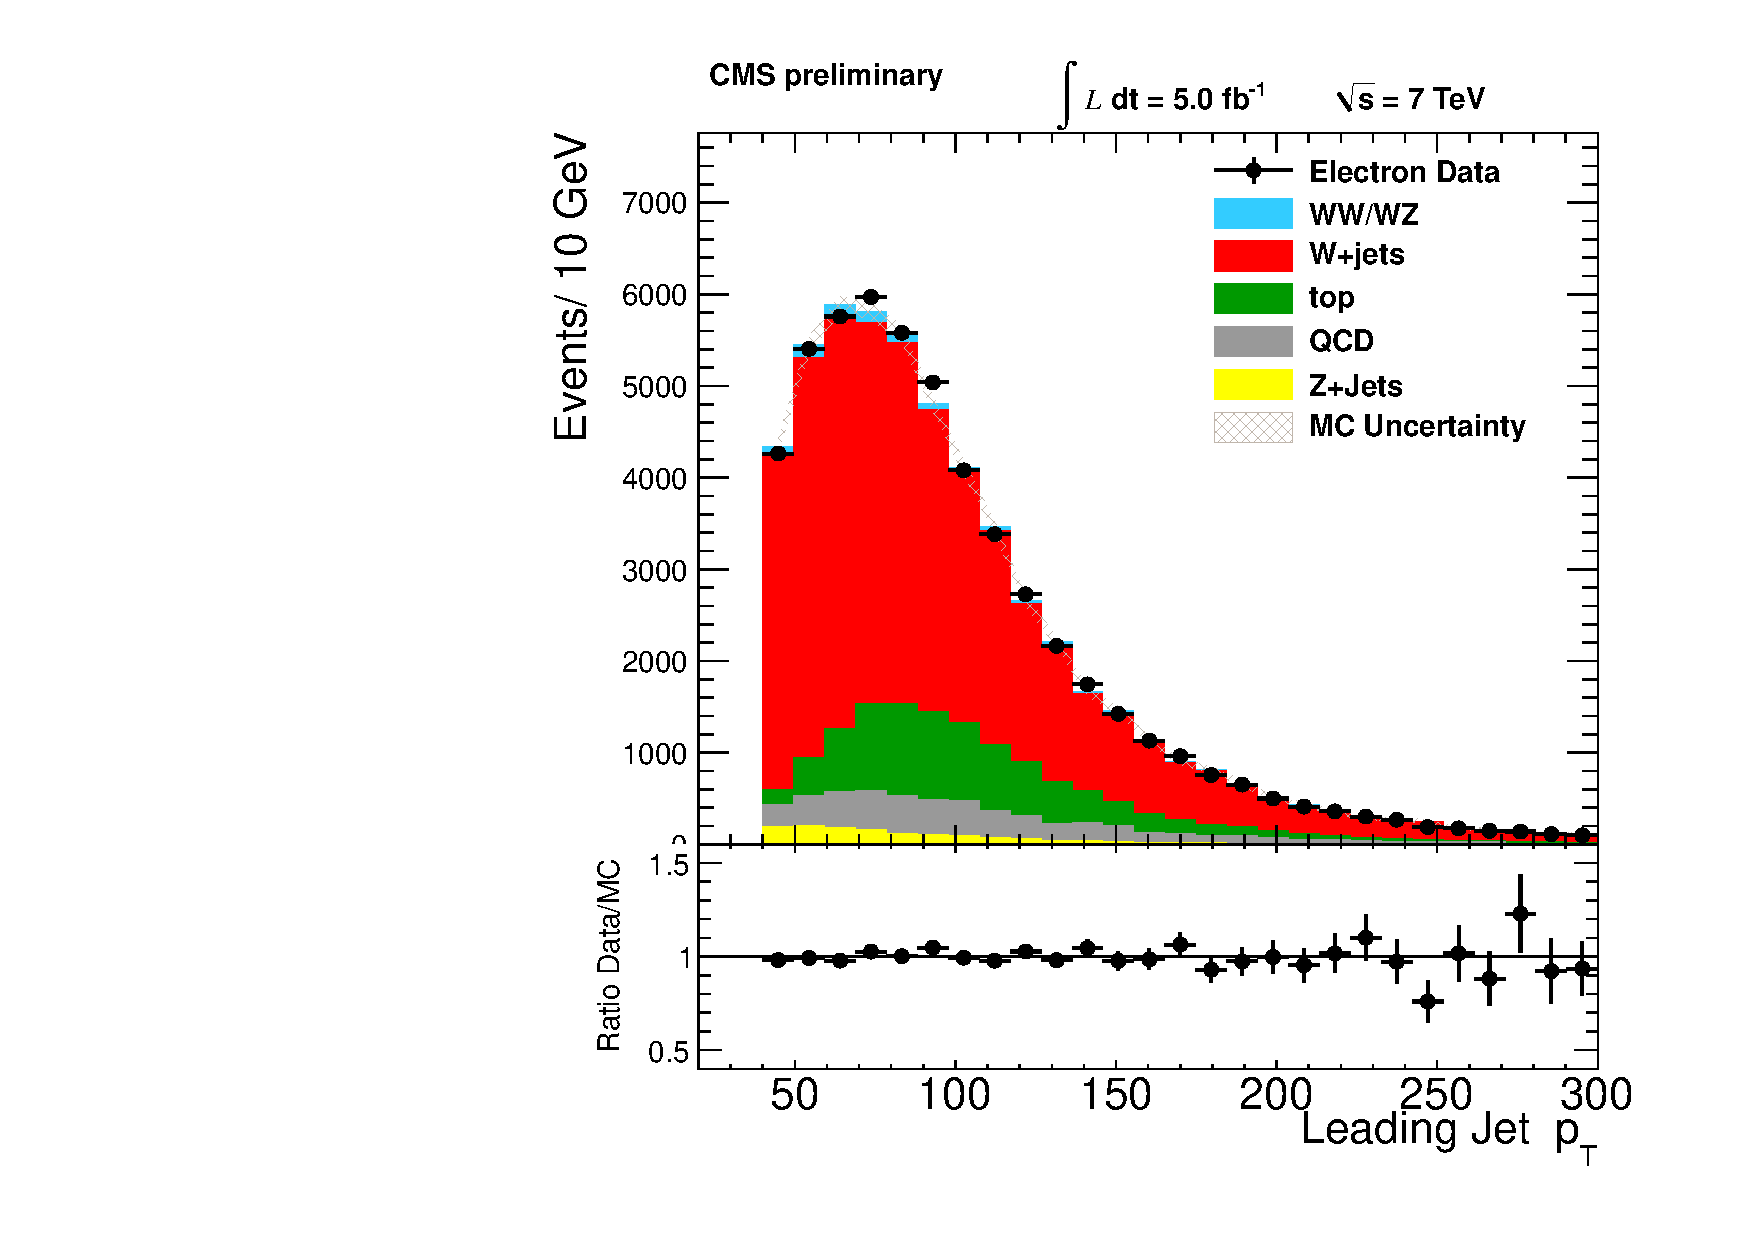
\includegraphics[width=0.49\textwidth]{figs/el_jetld_pt.pdf}
   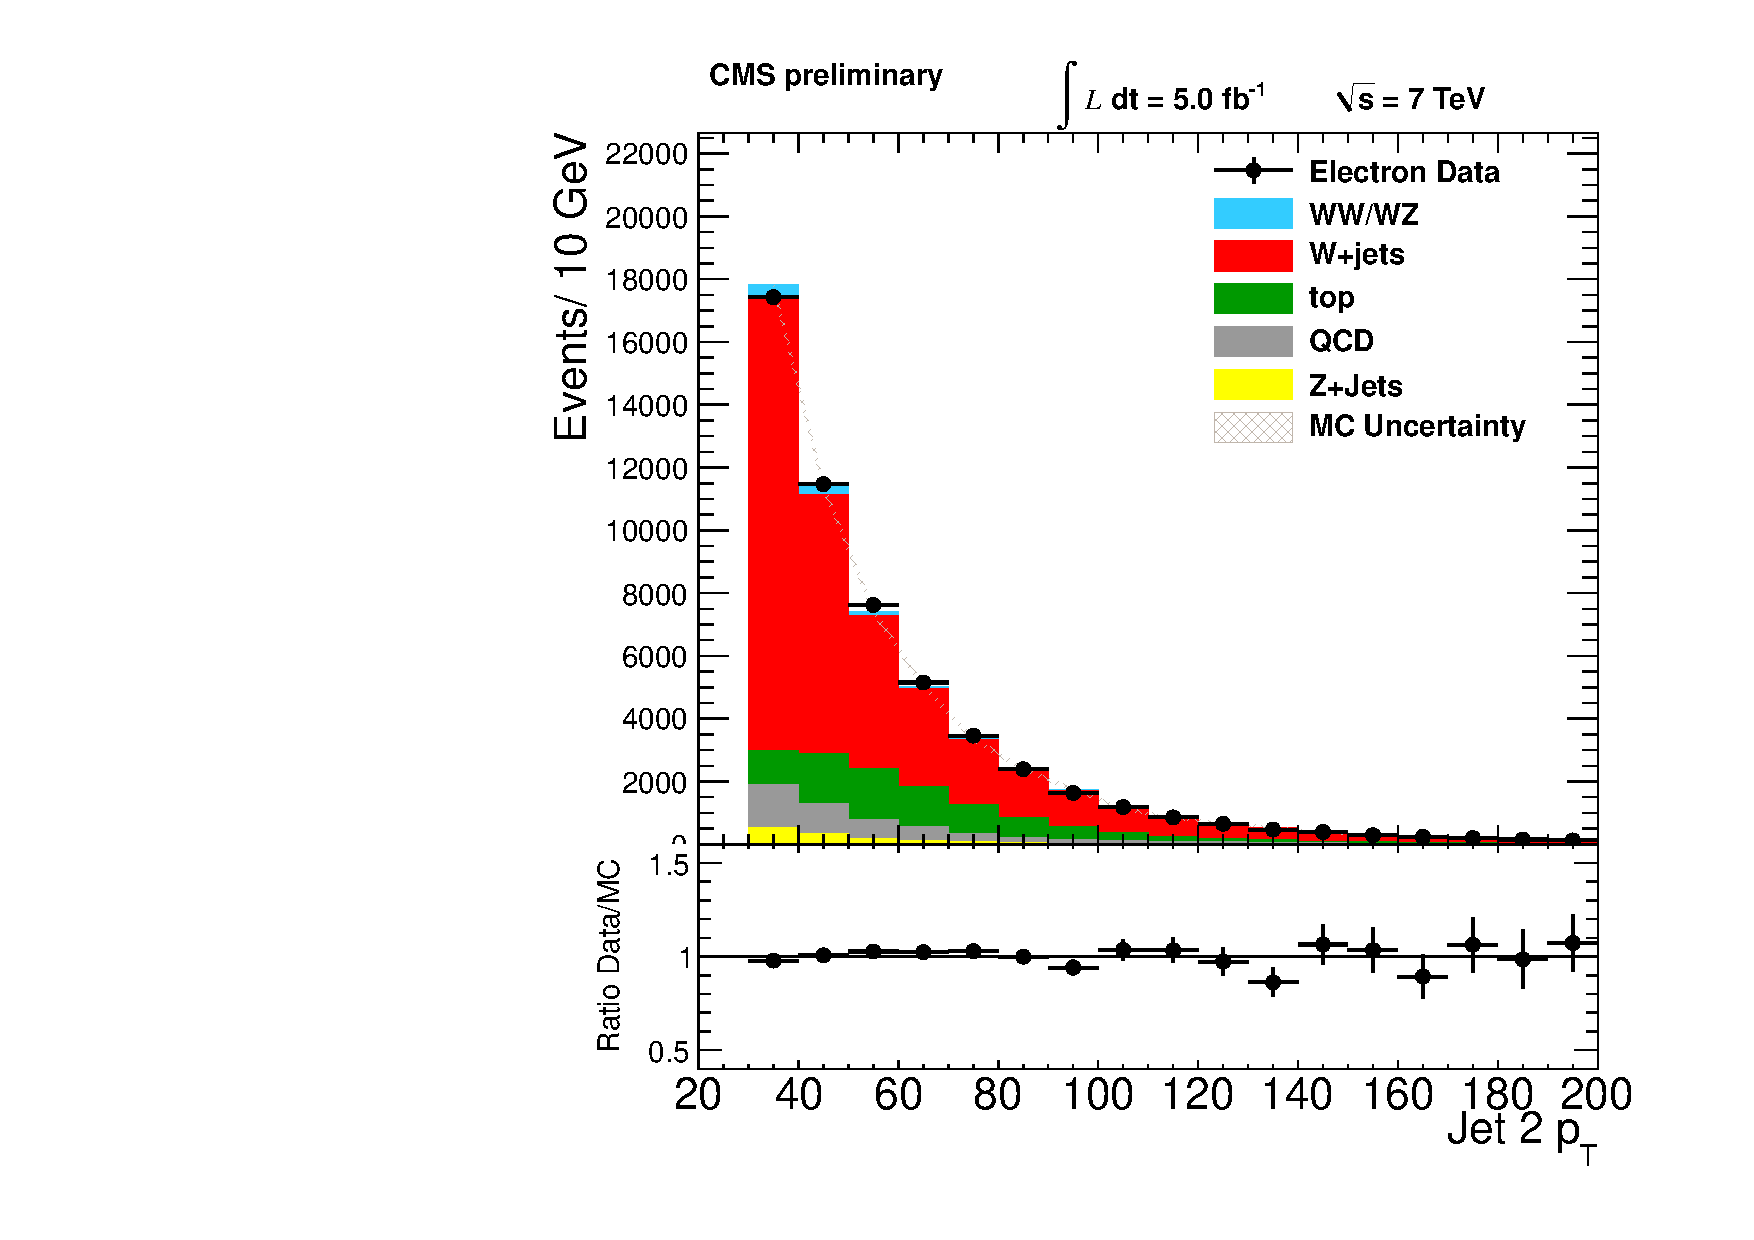
\includegraphics[width=0.49\textwidth]{figs/el_jetnt_pt.pdf}
   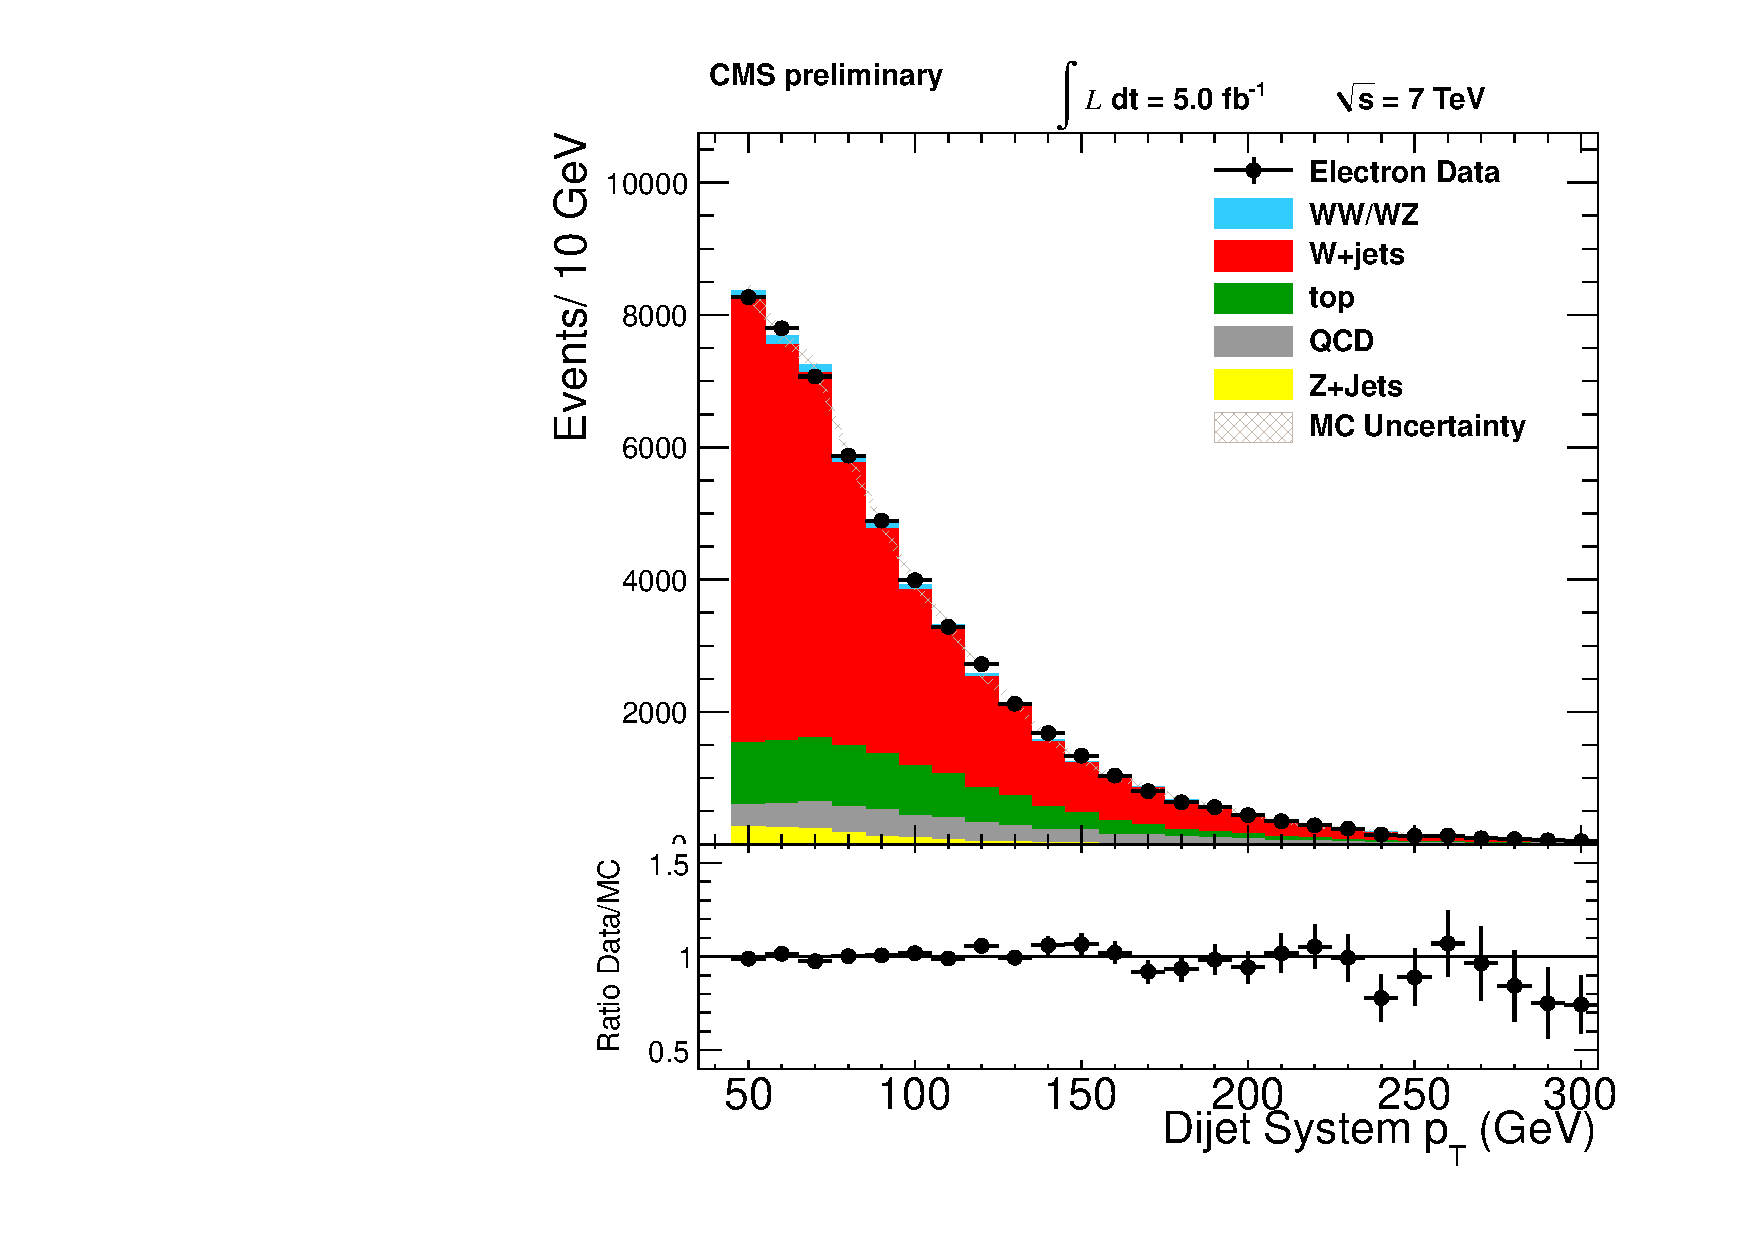
\includegraphics[width=0.49\textwidth]{figs/el_dijet_pt.pdf}
   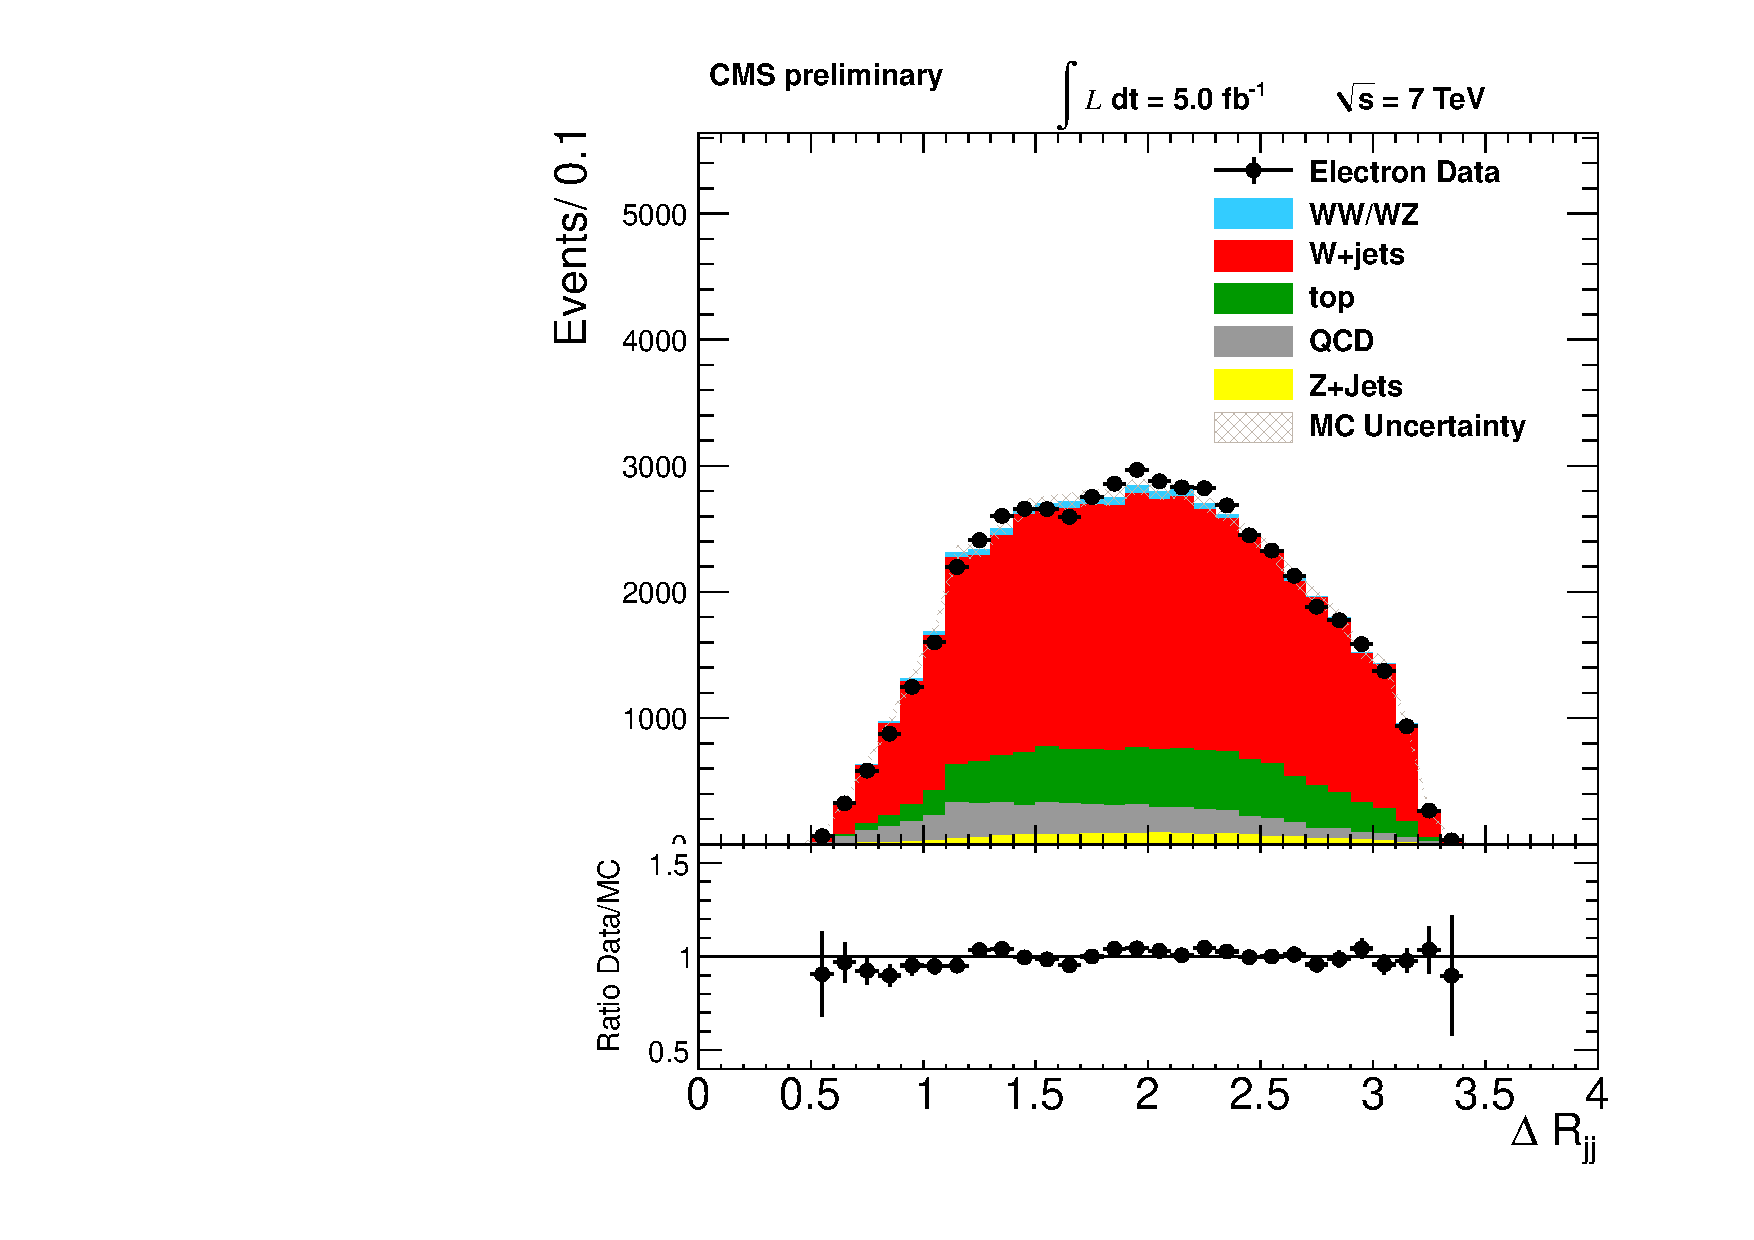
\includegraphics[width=0.49\textwidth]{figs/el_deltaRjj.pdf}
   \caption{Comparison of the distributions in data and MC for the
     electron plus jets event sample after event selection (upper
     left) of the transverse momentum of the leading jet, (upper
     right) of the transverse momentum of the second leading jet,
     (lower left) of the dijet transverse momentum, (lower right) of
     the dijet distance parameter $\Delta R= \sqrt{(\Delta
       \eta_{jj})^2 + (\Delta \phi_{jj})^2}$. The error bars on the
     data points are statistical only.  The relative normalization of
     the various MC samples are taken from the result of the fit to
     the \mjj spectrum.  }
 \end{figure*}


